\subsection{\texorpdfstring{同态 \(\mathbf{E}^* \otimes_{\mathbf{A}} \mathbf{F} \to \operatorname{Hom}_{\mathbf{A}}(\mathbf{E}, \mathbf{F})\)}{同态 \textbackslash mathbf\{E\}\^{}* \textbackslash otimes\_\{\textbackslash mathbf\{A\}\} \textbackslash mathbf\{F\} \textbackslash 到 \textbackslash operatorname\{Hom\}\_\{\textbackslash mathbf\{A\}\}(\textbackslash mathbf\{E\}, \textbackslash mathbf\{F\})}}

设 A、B 为两个环，E 为左A-模，F 为左B-模，G 为 (A, B)-双模。Z-模 \(\operatorname{Hom}_{\mathbf{A}}(\mathbf{E}, \mathbf{G})\) 典范地具有一个右B-模结构（§1，第14号），使得 \((u\beta)(x) = u(x)\beta\)（对 \(\beta \in \mathbf{B}\)、\(u \in \operatorname{Hom}_{\mathbf{A}}(\mathbf{E}, \mathbf{G})\)、\(x \in \mathbf{E}\)）。另一方面，\(\mathbf{G} \otimes_{\mathbf{B}} \mathbf{F}\) 典范地具有一个左A-模结构（§3，第4号）。我们将定义一个典范 \(\mathbf{Z}\)-同态

\[
\nu : \operatorname{Hom} _ {\mathbf {A}} (\mathrm{E}, \mathrm{G}) \otimes_ {\mathbf {B}} \mathrm{F} \rightarrow \operatorname{Hom} _ {\mathbf {A}} (\mathrm{E}, \mathrm{G} \otimes_ {\mathbf {B}} \mathrm{F}).\tag{7}
\]

为此，对于所有 \(y \in \mathbf{F}\) 以及所有 \(u \in \operatorname{Hom}_{\mathbf{A}}(\mathbf{E}, \mathbf{G})\)，我们考虑映射 \(\nu'(u, y): x \mapsto u(x) \otimes y\)（从 \(\mathbf{E}\) 到 \(\mathbf{G} \otimes_{\mathbf{B}} \mathbf{F}\)）。立即可以验证，\(\nu'(u, y)\) 是 A-线性的，且 \(\nu'\) 是从 \(\operatorname{Hom}_{\mathbf{A}}(\mathbf{E}, \mathbf{G}) \times \mathbf{F}\) 到 \(\operatorname{Hom}_{\mathbf{A}}(\mathbf{E}, \mathbf{G} \otimes_{\mathbf{B}} \mathbf{F})\) 的 Z-双线性映射；此外，对所有 \(\beta \in \mathbf{B}\)，\(\nu'(u\beta, y)\) 与 \(\nu'(u, \beta y)\) 相等，因为 \((u(x)\beta) \otimes y = u(x) \otimes (\beta y)\)。于是我们得出结论（§3，第1号，命题1）：存在所求的同态 \(\nu\)，使得 \(\nu(u \otimes y)\) 是 A-线性映射 \(x \mapsto u(x) \otimes y\)。

立即可以验证，若E是一个 \((\mathbf{A}, (\mathbf{C}_{i}^{\prime}) ; (\mathbf{D}_{j}^{\prime}))\) -多模，F是一个 \((\mathbf{B}, (\mathbf{C}_{h}^{\prime\prime}) ; (\mathbf{D}_{k}^{\prime\prime}))\) -多模，且G是一个 \((\mathbf{A}, (\mathbf{C}_{l}^{\prime\prime}) ; \mathbf{B}, (\mathbf{D}_{m}^{\prime\prime}))\) -多模，则映射(7)是一个 \(((\mathbf{D}_{j}^{\prime}), (\mathbf{C}_{h}^{\prime\prime}), (\mathbf{C}_{l}^{\prime\prime}) ; (\mathbf{C}_{i}^{\prime}), (\mathbf{D}_{k}^{\prime\prime}), (\mathbf{D}_{m}^{\prime\prime}))\) -多模同态。

命题2. (i) 当F是投射（相应地，有限生成投射）B-模时，典范同态(7)是单射（相应地，双射）。

\begin{enumerate}
\def\labelenumi{(\roman{enumi})}
\setcounter{enumi}{1}
\item
  当E是有限生成的投射A-模时，典范同态(7)是双射的。
\item
  固定E与G，对每个左B-模F，我们记
\end{enumerate}

\[
\mathrm{T} (\mathrm{F}) = \operatorname{Hom} _ {\mathrm{A}} (\mathrm{E}, \mathrm{G}) \otimes_ {\mathrm{B}} \mathrm{F}, \quad \mathrm{T} ^ {\prime} (\mathrm{F}) = \operatorname{Hom} _ {\mathrm{A}} (\mathrm{E}, \mathrm{G} \otimes_ {\mathrm{B}} \mathrm{F});
\]

对每个左B-模同态 \(u: \mathbf{F} \to \mathbf{F}'\)，我们记 \(\mathrm{T}(u) = 1 \otimes u\)（这里的1表示 \(\operatorname{Hom}_{\mathbf{A}}(\mathbf{E}, \mathbf{G})\) 的恒等映射），

\[
\mathrm{T} ^ {\prime} (u) = \operatorname{Hom} \left(\mathrm{l} _ {\mathbb {E}}, \mathrm{l} _ {\mathbb {G}} \otimes u\right);
\]

另一方面，我们用 \(\nu_{F}\) 代替 \(\nu\)。于是我们有以下引理：

引理1. 对于每个同态 \(u: \mathbf{F} \to \mathbf{F}'\) ，该图表

\[
\begin{array}{c c c} \mathrm{T(F)} & \xrightarrow {\nu_ {\mathrm{F}}} & \mathrm {T^ {\prime} (F)} \\ \mathrm{T(u)} \Big \downarrow & & \Big \downarrow \mathrm {T^ {\prime} (u)} \\ \mathrm {T(F^ {\prime})} & \xrightarrow {\nu_ {\mathrm {F^ {\prime}}}} & \mathrm {T^ {\prime} (F^ {\prime})} \end{array}\tag{8}
\]

是交换的。

验证是直接的。

引理2. 设 M, N 是 F 中的两个互补子模，i: M → F, j: N → F 为典范嵌入。图表

\begin{enumerate}
\def\labelenumi{(\arabic{enumi})}
\setcounter{enumi}{8}
\tightlist
\item
\end{enumerate}

\pandocbounded{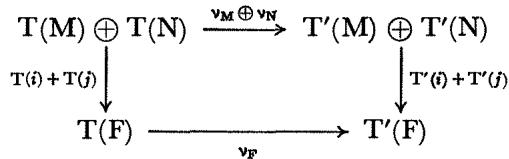
\includegraphics[keepaspectratio]{images/part002_2544dc0c.jpg}}

是可交换的，且竖直箭头是双射。

交换性由引理1得出，其余断言由§1第6号命题6的推论2以及§3第7号命题7得出。

引理3. 在引理2的假设下，\(\nu_{\mathrm{F}}\) 为单射（相应地，满射）的必要且充分条件是 \(\nu_{\mathrm{M}}\) 与 \(\nu_{\mathrm{N}}\) 皆然。

这由引理2及§1第6号命题6的推论1得出。

于是引理3连同§2第2号命题4表明，只需考虑F为自由模的情形。但若 \((b_{\mu})\) 是F的一组基，则 \(\operatorname{Hom}_{\mathbf{A}}(\mathbf{E}, \mathbf{G}) \otimes_{\mathbf{B}} \mathbf{F}\) 的每个元素都可唯一地写成 \(\sum_{\mu} u_{\mu} \otimes b_{\mu}\)，其中 \(u_{\mu} \in \operatorname{Hom}_{\mathbf{A}}(\mathbf{E}, \mathbf{G})\)（§3，第7号，命题7的推论1）；该元素在 \(\nu\) 下的像是 A-线性映射 \(x \mapsto \sum_{\mu} u_{\mu}(x) \otimes b_{\mu}\)；它不可能对所有 \(x \in \mathbf{E}\) 均为零，除非 \(u_{\mu}(x) = 0\)（对所有 \(x \in \mathbf{E}\) 与所有 \(\mu\) 成立），而这等价于 \(u_{\mu} = 0\)（对所有 \(\mu\)）；因此 \(\nu\) 是单射。当F还具有有限基时，引理3表明（通过对F的基中元素个数作归纳），要证明 \(\nu\) 是满射，只需就 \(F = B_s\) 的情形证明即可；但在此情形，(7) 式的两边都典范地等同于 \(\operatorname{Hom}_{\mathbf{A}}(\mathbf{E}, \mathbf{G})\)（§3，第4号，命题4），而 \(\nu\) 成为恒等映射。

\begin{enumerate}
\def\labelenumi{(\roman{enumi})}
\setcounter{enumi}{1}
\tightlist
\item
  为证明E为投射且有限生成时的命题，这次我们固定F与G，并对每个左A-模E记：
\end{enumerate}

\[
\mathrm{T} (\mathrm{E}) = \operatorname{Hom} _ {\mathrm{A}} (\mathrm{E}, \mathrm{G}) \otimes_ {\mathrm{B}} \mathrm{F}, \quad \mathrm{T} ^ {\prime} (\mathrm{E}) = \operatorname{Hom} _ {\mathrm{A}} (\mathrm{E}, \mathrm{G} \otimes_ {\mathrm{B}} \mathrm{F})
\]

并且，对于每一个左A模同态 \(v:\mathbf{E}\to\mathbf{E}^{\prime}\) ,

\[
\mathrm{T} (v) = \operatorname{Hom} (v, 1 _ {\mathbf {G}}) \otimes 1 _ {\mathbf {F}}, \quad \mathrm{T} ^ {\prime} (v) = \operatorname{Hom} (v, 1 _ {\mathbf {G}} \otimes 1 _ {\mathbf {F}});
\]

另一方面，我们用 \(\nu_{E}\) 代替 \(\nu\)。于是我们有以下两个引理：

引理4. 对于每个同态 \(v: \mathbf{E} \to \mathbf{E}'\) ，该图表

\[
\begin{array}{c c c} \mathrm{T} (\mathrm{E} ^ {\prime}) & \xrightarrow {\nu_ {\mathrm{E} ^ {\prime}}} & \mathrm{T} ^ {\prime} (\mathrm{E} ^ {\prime}) \\ \mathrm{T} (v) \Big \downarrow & & \Big \downarrow \mathrm{T} ^ {\prime} (v) \\ \mathrm{T} (\mathrm{E}) & \xrightarrow {\nu_ {\mathrm{E}}} & \mathrm{T} ^ {\prime} (\mathrm{E}) \end{array}\tag{10}
\]

是交换的。

引理5. 设 \(\mathbf{M}\) 与 \(\mathbf{N}\) 是 \(\mathbf{E}\) 中两个互补的子模，\(p: \mathbf{E} \to \mathbf{M}\)、\(q: \mathbf{E} \to \mathbf{N}\) 为典范投影。图表

\pandocbounded{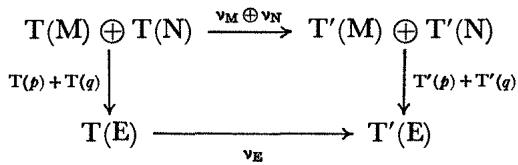
\includegraphics[keepaspectratio]{images/part002_a961576f.jpg}}

是可交换的，且竖直箭头是双射。

它们的证明与引理1和引理2相同，并用到§1第6号命题6的推论2、§2第1号命题1以及§3第7号命题7。

证明的余下部分随后按 (i) 的方式进行，并归结为 \(E = A_{s}\) 的情形；此时 (7) 式的两边典范地等同于 \(G \otimes_{B} F\)，而 \(\nu\) 成为恒等映射。

特别地，取 B = A 且 G 为 (A, A)-双模 \(_{s}A_{d}\)（§3，第4号），于是右A-模 \(\operatorname{Hom}_{\mathbf{A}}(\mathbf{E}, _{s}\mathbf{A}_{d})\) 就是E的对偶E*，并且 \((_{s}\mathbf{A}_{d}) \otimes_{\mathbf{A}} F\) 典范地等同于F（§3，第4号，命题4）。此时同态 (7) 成为典范Z-同态

\[
\theta : \mathrm{E} ^ {*} \otimes_ {\mathrm{A}} \mathrm{F} \rightarrow \operatorname{Hom} _ {\mathrm{A}} (\mathrm{E}, \mathrm{F})\tag{11}
\]

和 \(\theta (x^{*}\otimes y)\) 是E到F的线性映射

\[
x \mapsto \langle x, x ^ {*} \rangle y.
\]

注记（1）. §2 第6号命题12中给出的投射A模的刻画也可表述如下：对于左A模E为投射模，其充分必要条件为典范同态

\[
\theta_ {\mathbf {E}}: \mathrm{E} ^ {*} \otimes_ {\mathbf {A}} \mathrm{E} \rightarrow \operatorname{Hom} _ {\mathbf {A}} (\mathrm{E}, \mathrm{E}) = \operatorname{End} _ {\mathbf {A}} (\mathrm{E})
\]

使得 \(l_{E}\) 属于 \(\theta_{E}\) 的像。

推论. (i) 当F是投射（相应地，有限生成投射）模时，典范同态 (11) 是单射（相应地，双射）。

\begin{enumerate}
\def\labelenumi{(\roman{enumi})}
\setcounter{enumi}{1}
\tightlist
\item
  当E是有限生成投射模时，典范同态(11)是双射的。
\end{enumerate}

即使E与F都是有限生成的，\(\theta\) 也不一定满射，例 A = Z、E = F = Z/2Z 即说明这一点；(11) 式右端非零，但 \(E^{*} = 0\)。另一方面，可以给出E为自由模而 (11) 既非单射又非满射的例子（习题3(b)）。

当E具有有限基 \((e_i)\) 时，\(\theta^{-1}\)（\(\theta\) 的逆同构）可以如下显式求出。设 \((e_i^*)\) 为 \((e_i)\) 的对偶基（§2，第6号）；对所有 \(u \in \operatorname{Hom}(\mathbf{E}, \mathbf{F})\) 以及所有 \(x = \sum_{i} \xi_i e_i\)（其中 \(\xi_i \in \mathbf{A}\)），

\[
u (x) = \sum_ {i} \xi_ {i} u (e _ {i}) = \sum_ {i} \langle x, e _ {i} ^ {*} \rangle u (e _ {i})
\]

，从而 \(u = \sum_{i} \theta(e_i^* \otimes u(e_i))\)，换言之

\[
\theta^ {- 1} (u) = \sum_ {i} e _ {i} ^ {*} \otimes u (e _ {i}).\tag{12}
\]

特别地，若进一步有 F = E，则可看出 \(\theta_{E}^{-1}\) 把恒等映射 \(l_{E}\) 映为元素 \(\sum_{i} e_{i}^{*} \otimes e_{i}\)，因此该元素与E中所考虑的基 \((e_{i})\) 无关。

另一方面，注意当E是有限生成投射模时，\(\operatorname{End}_{\mathbf{A}}(\mathbf{E})\) 上的环结构可以通过 \(\theta_{E}^{-1}\) 转移到 \(E^{*}\otimes_{A}E\) 上；立即可以验证，对E中的 x, y 与 \(x^{*}, y^{*}\)（\(E^{*}\) 中的元素），在环 \(\operatorname{End}_{\mathbf{A}}(\mathbf{E})\) 中

\[
\theta_ {\mathbf {E}} (x ^ {*} \otimes x) \circ \theta_ {\mathbf {E}} (y ^ {*} \otimes y) = \theta_ {\mathbf {E}} ((y ^ {*} \langle y, x ^ {*} \rangle) \otimes x).\tag{13}
\]

注记 (2). 设 E 为右 A-模；在 (11) 中用 E* 替换 E，我们得到一个典范的 Z-同态

\[
\mathrm{E} ^ {* *} \otimes_ {\mathrm{A}} \mathrm{F} \rightarrow \operatorname{Hom} _ {\mathrm{A}} (\mathrm{E} ^ {*}, \mathrm{F}).\tag{14}
\]

另一方面，存在一个典范的 A-同态 \(c_{E}:E\to E^{**}\) ，由此得到一个 Z-同态 \(c_{E}\otimes l_{F}:E\otimes_{A}F\to E^{**}\otimes_{A}F\) ；将后者与同态 (14) 复合，我们从而得到一个典范的 Z-同态

\[
\theta^ {\prime}: \mathrm{E} \otimes_ {\mathrm{A}} \mathrm{F} \rightarrow \operatorname{Hom} _ {\mathrm{A}} (\mathrm{E} ^ {*}, \mathrm{F})\tag{15}
\]

使得 \(\theta'(x \otimes y)\) 是线性映射

\[
x ^ {*} \mapsto \langle x, x ^ {*} \rangle y.
\]

若 E 与 F 为投射模，则映射 (15) 是单射。因为 \(c_{E}\) 此时是单射（§2，第 7 号，命题 13 的推论 4），且由于 F 是投射的，Z-同态 \(c_{E} \otimes l_{F}: E \otimes_{A} F \to E^{**} \otimes_{A} F\) 也是单射（§3，第 7 号，命题 7 的推论 6）；最后，已见（命题 2）同态 (14) 是单射，由此得结论。

若 E 是投射且有限生成的，则映射 (15) 是双射，因为构成它的两个映射此时均为双射（§2，第 7 号，命题 13 的推论 4 及上文命题 2）。

\subsection{自同态的迹}

设 C 为交换环，E 为 C-模。映射 \((x^{*}, x) \mapsto \langle x, x^{*} \rangle\)（从 \(E^{*} \times E\) 到 C）是 C-双线性的，因为对所有 \(\gamma \in C\)，\(\langle \gamma x, x^{*} \rangle = \gamma \langle x, x^{*} \rangle\) 且 \(\langle x, x^{*} \gamma \rangle = \langle x, x^{*} \rangle \gamma\)；我们由此得到一个典范 C-线性映射

\[
\tau : \mathbf {E} ^ {*} \otimes_ {\mathbf {c}} \mathbf {E} \rightarrow \mathbf {C}\tag{16}
\]

使得 \(\tau(x^{*} \otimes x) = \langle x, x^{*} \rangle\)（§3，第5号）。现在再设E是有限生成的投射C-模；于是第2号的典范同构 (11) 是C-模同构，因此我们可以通过转移结构定义一个典范线性形式 \(\mathrm{Tr} = \tau \circ \theta_{\mathbf{E}}^{-1}\)（在C-模 \(\operatorname{End}_{\mathbf{C}}(\mathbf{E})\) 上）。对所有 \(u \in \operatorname{End}_{\mathbf{C}}(\mathbf{E})\)，标量 \(\operatorname{Tr}(u)\) 称为自同态 \(u\) 的迹；每个 \(u \in \operatorname{End}_{\mathbf{C}}(\mathbf{E})\) 都可以（一般以无穷多种方式）写成 \(x \mapsto \sum_{i} \langle x, x_{i}^{*} \rangle y_{i}\) 的形式，其中 \(x_{i}^{*} \in \mathbf{E}^{*}\)、\(y_{i} \in \mathbf{E}_{i}\)（依据第2号命题2的推论）；则

\[
\operatorname{Tr} (u) = \sum_ {i} \left\langle y _ {i}, x _ {i} ^ {*} \right\rangle \quad (\text { cf. } \S 1 0, \text { no. } 1 1).\tag{17}
\]

由定义，

\begin{enumerate}
\def\labelenumi{(\arabic{enumi})}
\setcounter{enumi}{17}
\tightlist
\item
\end{enumerate}

\[
\operatorname{Tr} (u + v) = \operatorname{Tr} (u) + \operatorname{Tr} (v)\tag{19}
\]

\[
\operatorname{Tr} (\gamma u) = \gamma \operatorname{Tr} (u)
\]

对 \(u, v\)（\(\operatorname{End}_{\mathbf{C}}(\mathbf{E})\) 中）及 \(\gamma \in \mathbf{C}\) 成立。此外：

命题3. 设 C 为交换环，E、F 为两个有限生成投射 C-模，且 \(u: \mathbf{E} \to \mathbf{F}\) 和 \(v: \mathbf{F} \to \mathbf{E}\) 为两个线性映射；则

\[
\operatorname{Tr} (v \circ u) = \operatorname{Tr} (u \circ v).\tag{20}
\]

映射 \((u, v) \mapsto \operatorname{Tr}(u \circ v)\) 与 \((u, v) \mapsto \operatorname{Tr}(v \circ u)\)（从

\[
\operatorname{Hom} _ {\mathbf {c}} (\mathbf {E}, \mathbf {F}) \times \operatorname{Hom} _ {\mathbf {c}} (\mathbf {F}, \mathbf {E})
\]

到C）都是 C-双线性的；因此只需在 u 形如 \(x \mapsto \langle x, a^{*} \rangle b\) 且 v 形如 \(y \mapsto \langle y, b^{*} \rangle a\)（其中 \(a \in E\)、\(a^{*} \in E^{*}\)、\(b \in F\)、\(b^{*} \in F^{*}\)）的情形验证 (20)。但此时 \(v \circ u\) 是映射 \(x \mapsto \langle x, a^{*} \rangle \langle b, b^{*} \rangle a\)，而 \(u \circ v\) 是映射 \(y \mapsto \langle y, b^{*} \rangle \langle a, a^{*} \rangle b\)。公式 (17) 表明 (20) 两端的值都等于 \(\langle a, a^{*} \rangle \langle b, b^{*} \rangle\)。

推论. 若 \(u_1, \ldots, u_p\) 是 \(\mathbf{E}\) 的自同态，则

\[
\operatorname{Tr} \left(u _ {1} \circ u _ {2} \circ \dots \circ u _ {p}\right) = \operatorname{Tr} \left(u _ {i} \circ u _ {i + 1} \circ \dots \circ u _ {p} \circ u _ {1} \circ \dots \circ u _ {i - 1}\right)
\]

对所有 \(1 \leqslant i \leqslant p\) 成立（“迹在循环置换下的不变性”）。

只需将 (20) 应用于乘积

\[
\left(u _ {1} \circ u _ {2} \circ \dots \circ u _ {i - 1}\right) \circ \left(u _ {i} \circ u _ {i + 1} \circ \dots \circ u _ {p}\right).
\]

注意另一方面，对于 E 的三个自同态 u、v、w，

\[
\operatorname{Tr} (u \circ v \circ w) = \operatorname{Tr} (u \circ w \circ v)
\]

不一定成立。

\subsection{\texorpdfstring{同态 \(\operatorname{Hom}_{\mathbb{C}}(\mathrm{E}_1, \mathrm{F}_1) \otimes_{\mathbb{C}} \operatorname{Hom}_{\mathbb{C}}(\mathrm{E}_2, \mathrm{F}_2) \to \operatorname{Hom}_{\mathbb{C}}(\mathrm{E}_1 \otimes_{\mathbb{C}} \mathrm{E}_2, \mathrm{F}_1 \otimes_{\mathbb{C}} \mathrm{F}_2)\)}{从 E1,F1 上的 Hom 与 E2,F2 上的 Hom 的 C 上张量积到相应张量积上的 Hom 的同态}}

设 C 为交换环，且 \(E_{1}\) , \(E_{2}\) , \(F_{1}\) , \(F_{2}\) 为四个 C-模；在 §3 第 5 号公式 (13) 中，我们定义了典范 C-模同态

\[
\lambda : \operatorname{Hom} (\mathbf {E} _ {1}, \mathbf {F} _ {1}) \otimes \operatorname{Hom} (\mathbf {E} _ {2}, \mathbf {F} _ {2}) \to \operatorname{Hom} (\mathbf {E} _ {1} \otimes \mathbf {E} _ {2}, \mathbf {F} _ {1} \otimes \mathbf {F} _ {2}). \tag {21}
\]

命题4. 当有序对 \((\mathbf{E}_1, \mathbf{E}_2)\)、\((\mathbf{E}_1, \mathbf{F}_1)\)、\((\mathbf{E}_2, \mathbf{F}_2)\) 之一由有限生成投射C-模组成时，典范同态 (21) 是双射。

显然，只需对有序对 \((\mathbf{E}_{1}, \mathbf{F}_{1})\) 与 \((\mathbf{E}_{1}, \mathbf{E}_{2})\) 证明即可。

我们先考虑有序对 \((\mathbf{E}_1, \mathbf{F}_1)\) 的情形；我们固定 \(\mathbf{E}_2, \mathbf{F}_1, \mathbf{F}_2\)，并对每个C-模记 \(\mathrm{T}(\mathbf{E}) = \mathrm{Hom}(\mathbf{E}, \mathbf{F}_1) \otimes_{\mathbb{C}} \mathrm{Hom}(\mathbf{E}_2, \mathbf{F}_2)\) 与 \(\mathrm{T}'(\mathbf{E}) = \mathrm{Hom}(\mathbf{E} \otimes \mathbf{E}_2, \mathbf{F}_1 \otimes \mathbf{F}_2)\)，且对每个C-同态 \(v: \mathbf{E} \to \mathbf{E}'\)，

\[
\mathrm{T} (v) = \operatorname{Hom} (v, \mathrm{l} _ {\mathrm{F} _ {1}}) \otimes \mathrm{l} _ {\operatorname{Hom} (\mathrm{E} _ {2}, \mathrm{F} _ {2})}
\]

和

\[
\mathrm{T} ^ {\prime} (v) = \operatorname{Hom} (v \otimes 1 _ {\mathbb {E} _ {2}}, 1 _ {\mathbf {F} _ {1} \otimes \mathbf {F} _ {2}}).
\]

于是引理4与引理5（第2号）（其中v换成了λ）成立，且可用完全类似的方法证明。

接下来我们固定 \(\mathbf{E}_2\) 与 \(\mathbf{F}_2\)，这次对每个C-模 \(\mathbf{F}\) 记 \(\mathrm{T}(\mathbf{F}) = \mathrm{Hom}(\mathbf{C},\mathbf{F})\otimes_{\mathbb{C}}\mathrm{Hom}(\mathbf{E}_2,\mathbf{F}_2)\) 与 \(\mathrm{T}'(\mathrm{F}) = \mathrm{Hom}(\mathbf{C}\otimes \mathbf{E}_2,\mathbf{F}\otimes \mathbf{F}_2)\)，且对每个C-同态 \(u:\mathrm{F}\to \mathrm{F}'\)，

\[
\mathrm{T} (u) = \operatorname{Hom} (\mathrm{l} _ {\mathbf {c}}, u) \otimes \mathrm{l} _ {\operatorname{Hom} (\mathbb {E} _ {2}, \mathrm{F} _ {2})}
\]

和

\[
\mathrm{T} ^ {\prime} (u) = \operatorname{Hom} (\mathrm{l} _ {\mathrm{c}} \otimes \mathrm{l} _ {\mathrm{E} _ {2}}, u \otimes \mathrm{l} _ {\mathrm{F} _ {2}}).
\]

这次可立即验证引理1与引理2（第2号）（其中 \(\lambda\) 处处代替 \(\nu\)）成立。

这样，我们先在 \(E_{1} = C\) 且 \(F_{1}\) 为投射且有限生成的情形证明该命题。第2号的论证（基于引理1与引理2）连同上述说明，把它归结为在 \(F_{1} = C\) 时证明该命题；于是 \(\operatorname{Hom}(E_{1}, F_{1})\)、\(E_{1} \otimes E_{2}\) 与 \(F_{1} \otimes F_{2}\) 分别等同于C、\(E_{2}\) 与 \(F_{2}\)（§3，第4号，命题4）；从而 (21) 式的两边都典范地等同于 \(\operatorname{Hom}(\mathbf{E}_{2},\mathbf{F}_{2})\)，且在这些等同之后，可验证 \(\lambda\) 成为恒等映射。

我们现在假设 \(F_{1}\) 是投射且有限生成的；第2号的论证（这次依赖引理4与引理5）把 \(E_{1}\) 为任意有限生成投射模时的证明归结为 \(E_{1} = C\) 的情形，即归结为已处理的第一种情形。

对于有序对 \((\mathbf{E}_{1}, \mathbf{E}_{2})\) ，过程类似，这次两次应用引理4和5；细节留给读者。

注意当 \(\mathbf{E}_1 = \mathbf{C}^{(I)}\)、\(\mathbf{E}_2 = \mathbf{C}^{(J)}\) 是自由模（不论是否有限生成）时，有 \(\operatorname{Hom}(\mathbf{E}_1, \mathbf{F}_1) = \mathbf{F}_1^{\mathrm{I}}\)、\(\operatorname{Hom}(\mathbf{E}_2, \mathbf{F}_2 = \mathbf{F}_2^{\mathrm{J}}\) 以及

\[
\operatorname{Hom} \left(\mathrm{E} _ {1} \otimes \mathrm{E} _ {2}, \mathrm{F} _ {1} \otimes \mathrm{F} _ {2}\right) = \left(\mathrm{F} _ {1} \otimes \mathrm{F} _ {2}\right) ^ {\mathrm{I} \times \mathrm{J}}
\]

（这在典范同构的意义下成立），且 (21) 此时就是§3第7号中典范同态 (22) 的一个特例。

当 \(E_{2} = C\) 时，把 \(\operatorname{Hom}(E_{2}, F_{2})\) 与 \(F_{2}\)、\(E_{1} \otimes E_{2}\) 与 \(E_{1}\) 等同后，典范同态 (21) 给出一个典范同态

\[
\operatorname{Hom} (\mathrm{E}, \mathrm{F}) \otimes \mathrm{G} \rightarrow \operatorname{Hom} (\mathrm{E}, \mathrm{F} \otimes \mathrm{G})\tag{22}
\]

对任意三个C-模E、F、G，它恰好是 \(\mathbf{A} = \mathbf{B} = \mathbf{C}\) 时第2号中的同态 (7)。

注意当 \(\mathbf{F} = \mathbf{C}\) 时，典范同态 (22) 再次给出交换环情形下的 (11)（第2号）。

现在假设 \(\mathbf{F}_1 = \mathbf{F}_2 = \mathbf{C}\)；由于 \(\mathbf{F}_1 \otimes \mathbf{F}_2\) 与 \(\mathbf{C}\) 等同，这次得到一个典范同态

\[
\mu : \mathbf {E} ^ {*} \otimes \mathbf {F} ^ {*} \rightarrow (\mathbf {E} \otimes \mathbf {F}) ^ {*}\tag{23}
\]

对于两个 C-模 E, F；对 \(x^{*} \in \mathbf{E}^{*}\)、\(y^{*} \in \mathbf{F}^{*}\)，\(x^{*} \otimes y^{*}\) 在典范同态 (23) 下的像是线性形式 \(u\)（\(\mathbf{E} \otimes \mathbf{F}\) 上的），满足

\[
u (x \otimes y) = \langle x, x ^ {*} \rangle \langle y, y ^ {*} \rangle .\tag{24}
\]

此外，若 \(E_{1}\) , \(E_{2}\) , \(F_{1}\) , \(F_{2}\) 是四个 C-模， \(f: E_{1} \rightarrow E_{2}\) , \(g: F_{1} \rightarrow F_{2}\) 是两个线性映射，则由 (24) 立即得出图表

\[
\begin{array}{c} \mathrm{E} _ {2} ^ {*} \otimes \mathrm{F} _ {2} ^ {*} \xrightarrow {\mu} (\mathrm{E} _ {2} \otimes \mathrm{F} _ {2}) ^ {*} \\ t _ {f} \otimes t _ {g} \Biggl \downarrow \qquad \qquad \qquad \qquad \qquad \qquad \qquad \qquad \qquad \qquad \qquad \qquad \qquad \qquad \qquad \qquad \qquad \qquad \qquad \qquad \qquad \qquad \qquad \qquad \qquad \qquad \qquad \qquad \qquad \qquad \qquad \qquad \qquad \qquad \\ \mathrm{E} _ {1} ^ {*} \otimes \mathrm{F} _ {1} ^ {*} \xrightarrow {\mu} (\mathrm{E} _ {1} \otimes \mathrm{F} _ {1}) ^ {*} \end{array}\tag{25}
\]

是交换的。

推论 1. 若模 E, F 中有一个是投射且有限生成的，则典范同态 (23) 是双射。

推论2. 设 \(\mathbf{E}_1, \mathbf{E}_2\) 是两个有限生成的投射C-模，\(u_1\) 是 \(\mathbf{E}_1\) 的一个自同态，\(u_2\) 是 \(\mathbf{E}_2\) 的一个自同态；则

\[
\operatorname{Tr} (u _ {1} \otimes u _ {2}) = \operatorname{Tr} (u _ {1}) \operatorname{Tr} (u _ {2}).\tag{26}
\]

由线性性，只需考虑 \(u_{1}\) 形如 \(x_{1} \mapsto \langle x_{1}, x_{1}^{*} \rangle y_{1}\) 且 \(u_{2}\) 形如 \(x_{2} \mapsto \langle x_{2}, x_{2}^{*} \rangle y_{2}\) 的情形；则 \(x_{1} \otimes x_{2}\) 在 \(u_{1} \otimes u_{2}\) 下的像按定义为

\[
\langle x _ {1}, x _ {1} ^ {*} \rangle \langle x _ {2}, x _ {2} ^ {*} \rangle (y _ {1} \otimes y _ {2}) = \langle x _ {1} \otimes x _ {2}, x _ {1} ^ {*} \otimes x _ {2} ^ {*} \rangle (y _ {1} \otimes y _ {2})
\]

其中 \(x_{1}^{*}\otimes x_{2}^{*}\) 在 \(\mu\) 下典范地等同于 \((\mathrm{E}_{1}\otimes\mathrm{E}_{2})^{*}\) 中的一个元素。由于 \(\langle y_{1}\otimes y_{2},x_{1}^{*}\otimes x_{2}^{*}\rangle=\langle y_{1},x_{1}^{*}\rangle\langle y_{2},x_{2}^{*}\rangle\)，公式 (26) 在此情形由 (17) 得出。

注记。若E、F、G是任意三个C-模，则容易验证图表

\[
\begin{array}{c} \mathrm{E} ^ {*} \otimes \mathrm{F} ^ {*} \otimes \mathrm{G} ^ {*} \xrightarrow {\mu \otimes 1} (\mathrm{E} \otimes \mathrm{F}) ^ {*} \otimes \mathrm{G} ^ {*} \\ 1 \otimes \mu \Biggl \downarrow \\ \mathrm{E} ^ {*} \otimes (\mathrm{F} \otimes \mathrm{G}) ^ {*} \xrightarrow [ \mu ]{} (\mathrm{E} \otimes \mathrm{F} \otimes \mathrm{G}) ^ {*} \end{array}\tag{27}
\]

是交换的，这可由公式(24)得出。

我们还注意到，在不假设C-模E、F有任何条件的情况下，存在典范同构

\begin{enumerate}
\def\labelenumi{(\arabic{enumi})}
\setcounter{enumi}{27}
\tightlist
\item
\end{enumerate}

\[
(\mathbf {E} \otimes \mathbf {F}) ^ {*} \rightarrow \operatorname{Hom} (\mathbf {E}, \mathbf {F} ^ {*})\tag{29}
\]

\[
(\mathbf {E} \otimes \mathbf {F}) ^ {*} \rightarrow \operatorname{Hom} (\mathbf {F}, \mathbf {E} ^ {*})
\]

它们即第1号中取 \(\mathbf{G} = \mathbf{C}\)、\(\mathbf{A} = \mathbf{B} = \mathbf{C}\) 时的同构 (6) 与 (5)。

这样，在 \(E \times F\) 上的双线性形式、从E到 \(F^{*}\) 的同态与从F到 \(E^{*}\) 的同态之间，就定义了一个典范的一一对应：若 u（相应地 v）是从E到 \(F^{*}\)（相应地，从F到 \(E^{*}\)）的同态，则相应的双线性形式由下式给出

\[
(x, y) \mapsto \langle y, u (x) \rangle \quad (\text { resp. } (x, y) \mapsto \langle x, v (y) \rangle).
\]

\section{标量环的扩张}

\subsection{模的标量环的扩张}

设 A、B 为两个环，\(\rho: \mathbf{A} \to \mathbf{B}\) 为环同态；我们考虑由该同态定义的右A-模 \(\rho^{*}(B_{d})\)（§1，第13号）；这个A-模还具有左B-模结构，即 \(B_{s}\) 的结构，并且由于 \(b'(b\rho(a)) = (b'b)\rho(a)\)（对 \(a \in \mathbf{A}\) 及B中的 \(b\)、\(b'\)），B上的这两个模结构是相容的（§1，第14号）。这使我们可以对每个左A-模E，在张量积 \(\rho_{*}(B_{d}) \otimes_{\mathbf{A}} \mathbf{E}\) 上定义一个左B-模结构，使得 \(\beta'(\beta \otimes x) = (\beta'\beta) \otimes x\)（对B中的 \(\beta\)、\(\beta'\) 及 \(x \in \mathbf{E}\)）（§3，第3号）。这个左B-模称为借助 \(\rho\) 把标量环扩张到B而由E导出的模，记作 \(\rho^{*}(\mathbf{E})\) 或 \(\mathrm{E}_{(\mathbf{B})}\)（不致混淆时）。

对每个左A-模E，映射 \(\phi: x \mapsto 1 \otimes x\)（从E到A-模 \(\rho_*(\rho^*(\mathbf{E}))\)）是A-线性的，且集合 \(\phi(\mathbf{E})\) 生成B-模 \(\rho^*(\mathbf{E})\)。进而，对每个左B-模F与每个A-线性映射 \(f\)（从E到A-模 \(\rho_*(\mathbf{F})\)），存在唯一的B-线性映射 \(\tilde{f}\)（从 \(\rho^*(\mathbf{E})\) 到F），使得 \(\tilde{f}(1 \otimes x) = f(x)\)（对所有 \(x \in \mathbf{E}\)）。

B 可借助 \(\rho\) 视为一个 (B, A)-双模；于是存在一个典范的 Z-模同构

\[
\operatorname{Hom} _ {\mathbf {B}} (\mathbf {B} \otimes_ {\mathbf {A}} \mathbf {E}, \mathbf {F}) \rightarrow \operatorname{Hom} _ {\mathbf {A}} (\mathbf {E}, \operatorname{Hom} _ {\mathbf {B}} (\mathbf {B} _ {s}, \mathbf {F}))\tag{1}
\]

这正如§4第1号命题1所示。但左A-模 \(\mathrm{Hom}_{\mathbf{B}}(\mathbf{B}_{s},\mathbf{F})\) 典范地等同于 \(\rho^{*}(\mathbf{F})\)：因为按定义（§1，第14号），对元素 \(y\in \mathbf{F}\) 对应着同态 \(\theta (y)\colon \mathbf{B}_s\to \mathbf{F}\)，它满足 \((\theta (y))(1) = y\)；于是对所有 \(\lambda \in \mathbf{A}\)，对 \(\rho (\lambda)y\in \mathbf{F}\) 对应着同态 \(\mu \mapsto \mu \rho (\lambda)y\)（从 \(\mathbf{B}_s\) 到 \(\mathbf{F}\) 的），它正是 \(\lambda \theta (y)\)（对 \(\mathrm{Hom}_{\mathbf{B}}(\mathbf{B}_{s},\mathbf{F})\) 的左A-模结构而言）（§1，第14号）。利用这一等同，我们因此得到一个典范Z-模同构，即 (1) 的逆

\[
\delta : \operatorname{Hom} _ {\mathbf {A}} (\mathbf {E}, \rho_ {*} (\mathbf {F})) \rightarrow \operatorname{Hom} _ {\mathbf {B}} (\rho^ {*} (\mathbf {E}), \mathbf {F})\tag{2}
\]

并且由定义立即得出，若 \(\delta(f) = \bar{f}\)，则 \(\bar{f}(1 \otimes x) = f(x)\)（对所有 \(x \in \mathbf{E}\)）。特别地，映射 \(\phi_{\mathbb{E}}: x \mapsto 1 \otimes x\) 恰好就是

\[
\phi_ {\mathbf {E}} = \delta^ {- 1} (1 _ {\rho^ {*} (\mathbf {E})}).\tag{3}
\]

因此，命题1得证。该映射 \(\phi_{\mathbf{E}}: \mathbf{E} \to \rho_{*}(\rho^{*}(\mathbf{E}))\) 被称为典范的。

注. (1) 命题1表明，由 \(\mathbf{E}_{(\mathbf{B})}\) 与 \(\phi_{\mathbb{E}}\) 组成的有序对是泛映射问题（集合论，IV，§3，第1号）的一个解，其中 \(\Sigma\) 是左B-模结构的物种（态射为B-线性映射），而 \(\alpha\)-映射是E到某个B-模中的A-线性映射。

\begin{enumerate}
\def\labelenumi{(\arabic{enumi})}
\setcounter{enumi}{1}
\item
  若E是一个 \((\mathbf{A}, (\mathbf{C}_{i}^{\prime}); (\mathbf{D}_{j}^{\prime}))\) -多模且F是一个 \((\mathbf{B}, (\mathbf{C}_{h}^{\prime\prime}); (\mathbf{D}_{k}^{\prime\prime}))\) -多模，则同构(2)关于两边的 \(((\mathbf{D}_{j}^{\prime}), (\mathbf{C}_{h}^{\prime\prime}); (\mathbf{C}_{i}^{\prime}), (\mathbf{D}_{k}^{\prime\prime}))\) -多模结构是线性的（§1，第14号及§3，第4号）。
\item
  设E为左A-模，a为A的双边理想，且 \(\rho:A\to A/a\) 为典范同态。在§3第6号命题6推论2的记号下，A-模E/aE被a零化，因此典范地具有左(A/a)-模结构（§1，第12号）；显然，§3第6号命题6推论2中定义的典范映射 \(\pi:\rho^{*}(E)\to E/aE\) 对于(A/a)-模结构是同构。
\end{enumerate}

推论。设E，E'为两个左A-模；对每个A-线性映射u: E → E'，v = l\_B ⊗ u是使下图交换的唯一B-线性映射

\pandocbounded{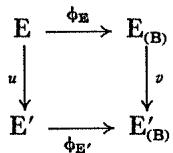
\includegraphics[keepaspectratio]{images/part002_74d11806.jpg}}

（其中 \(\phi_{\mathbf{E}}\) 与 \(\phi_{\mathbf{E}'}\) 是典范映射）。

只需将命题1应用于A-同态 \(\phi_{\mathbf{E}'} \circ u: \mathbf{E} \to \mathbf{E}_{(\mathbf{B})}'\)。

上述推论中定义的映射 \(v\) 记作 \(\rho^{*}(u)\) 或 \(u_{(B)}\)。若 \(E''\) 是第三个左A-模且 \(v: E' \to E''\) 为A-线性映射，则显然

\[
\left(v \circ u\right) _ {(\mathbf {B})} = v _ {(\mathbf {B})} \circ u _ {(\mathbf {B})}.
\]

模的算子环的扩张是一种可传递的运算；确切地说：

命题2. 设 \(\rho: \mathbf{A} \to \mathbf{B}\) , \(\sigma: \mathbf{B} \to \mathbf{C}\) 是环同态。对每个左A-模E，存在唯一的C-同态

\[
\sigma^ {*} (\rho^ {*} (\mathrm{E})) \rightarrow (\sigma \circ \rho) ^ {*} (\mathrm{E})\tag{4}
\]

它把 \(1 \otimes (1 \otimes x)\) 映为 \(1 \otimes x\)（对所有 \(x \in E\)），且该同态是双射。

\(\sigma^{*}(\rho^{*}(\mathbf{E}))\) 与 \((\sigma \circ \rho)^{*}(\mathbf{E})\) 的底层Z-模分别是 \(\mathbf{C} \otimes_{\mathbf{B}} (\mathbf{B} \otimes_{\mathbf{A}} \mathbf{E})\) 与 \(\mathbf{C} \otimes_{\mathbf{A}} \mathbf{E}\)。存在一个典范Z-同构 \(\mathbf{C} \otimes_{\mathbf{B}} (\mathbf{B} \otimes_{\mathbf{A}} \mathbf{E}) \to (\mathbf{C} \otimes_{\mathbf{B}} \mathbf{B}) \otimes_{\mathbf{A}} \mathbf{E}\) （§ 3，第8号，命题8），它对于两侧的左C-模结构也是C-同构。此外，C-模C ⊗B B在映射γ ⊗ β到γσ(β)的同构下典范地等同于C-模Cs（§ 3，第4号，命题4），并且该同构也是对于由ρ定义的C ⊗B B上的右A-模结构和由σ ∘ ρ定义的C上的右A-模结构的同构。因此，存在一个典范同构

\[
(\mathbf {C} \otimes_ {\mathbf {B}} \mathbf {B}) \otimes_ {\mathbf {A}} \mathbf {E} \rightarrow \mathbf {C} \otimes_ {\mathbf {A}} \mathbf {E}
\]

于是就得到；将它与同构

\[
\mathbf {C} \otimes_ {\mathbf {B}} (\mathbf {B} \otimes_ {\mathbf {A}} \mathbf {E}) \rightarrow (\mathbf {C} \otimes_ {\mathbf {B}} \mathbf {B}) \otimes_ {\mathbf {A}} \mathbf {E}
\]

复合，就得到所需的典范同构。

若 \(\phi, \phi'\) 和 \(\phi''\) 分别记典范映射 \(E \to \rho^*(E)\) , \(\rho^*(E \to) \sigma^*(\rho^*(E))\) 和 \(E \to (\sigma \circ \rho)^*(E)\) ,则在命题2的典范同构下，\(\phi' \circ \phi\) 与 \(\phi''\) 等同。

命题3. 设A，B为两个交换环， \(\rho: \mathbf{A} \to \mathbf{B}\) 为环同态，且 E、E' 是两个 A-模。存在唯一的 B-同态

\[
\mathbf {E} _ {(\mathbf {B})} \otimes_ {\mathbf {B}} \mathbf {E} _ {(\mathbf {B})} ^ {\prime} \rightarrow (\mathbf {E} \otimes_ {\mathbf {A}} \mathbf {E} ^ {\prime}) _ {(\mathbf {B})}\tag{5}
\]

它把 \((1 \otimes x) \otimes (1 \otimes x')\) 映为 \(1 \otimes (x \otimes x')\)（对 \(x \in \mathbf{E}\)、\(x' \in \mathbf{E}'\)），且该同态是双射。

（5）的左边可写成 \((\mathbf{B} \otimes_{\mathbf{A}} \mathbf{E}) \otimes_{\mathbf{B}} (\mathbf{B} \otimes_{\mathbf{A}} \mathbf{E}')\)，且（因A与B交换）与 \((\mathbf{E} \otimes_{\mathbf{A}} \mathbf{B}) \otimes_{\mathbf{B}} (\mathbf{B} \otimes_{\mathbf{A}} \mathbf{E}')\) 等同；后一个乘积依次等同于 \(\mathbf{E} \otimes_{\mathbf{A}} (\mathbf{B} \otimes_{\mathbf{B}} \mathbf{B}) \otimes_{\mathbf{A}} \mathbf{E}'\) , \(\mathbf{E} \otimes_{\mathbf{A}} (\mathbf{B} \otimes_{\mathbf{A}} \mathbf{E}')\) , \(\mathbf{E} \otimes_{\mathbf{A}} (\mathbf{E}' \otimes_{\mathbf{A}} \mathbf{B})\) ，最终等同于 \((\mathbf{E} \otimes_{\mathbf{A}} \mathbf{E}') \otimes_{\mathbf{A}} \mathbf{B}\) ，这利用了张量积的结合性（§3，第8号，命题8）、§3第4号命题4以及A与B的交换性。所需的同构是这些相继的典范同构的复合。

显然，若S是E的一个生成系，则S在典范映射 \(E \rightarrow E_{(B)}\) 下的像是 \(E_{(B)}\) 的一个生成系；特别地，若E是有限生成的A-模，则 \(E_{(B)}\) 是有限生成的B-模。

命题4. 设E是具有基 \((a_{\lambda})_{\lambda \in L}\) 的A-模；若 \(\phi : x \mapsto 1 \otimes x\) 是E到 \(\rho^{*}(\mathbf{E})\) 的典范映射，则 \((\phi(a_{\lambda}))_{\lambda \in L}\) 是 \(\rho^{*}(\mathbf{E})\) 的一组基。若 \(\rho\) 是单射，则 \(\phi\) 亦然。

第一个断言直接由§3第7号命题7的推论1得出。此外，对A中元素的每个有限支撑族 \((\xi_{\lambda})_{\lambda \in L}\)，有 \(\phi\left(\sum_{\lambda \in L} \xi_{\lambda} a_{\lambda}\right) = \sum_{\lambda \in L} \rho(\xi_{\lambda}) \phi(a_{\lambda})\)，因而关系 \(\phi\left(\sum_{\lambda \in L} \xi_{\lambda} a_{\lambda}\right) = 0\) 等价于 \(\rho(\xi_{\lambda}) = 0\)（对所有 \(\lambda \in L\)），由此得出第二个断言。

推论. 对每个投射A-模E，B-模 \(\rho^{*}(\mathbf{E})\) 是投射的。若进一步 \(\rho\) 是单射，则E到 \(\rho^{*}(\mathbf{E})\) 的典范映射是单射。

由假设，存在一个包含E的自由A-模M，且E在M中有一个补子模F。由§3第7号命题7直接可得，\(\mathbf{M}_{(\mathbf{B})}\) 等同于 \(\mathbf{E}_{(\mathbf{B})}\) 与 \(\mathbf{F}_{(\mathbf{B})}\) 的直和，且若 \(\phi\) 和 \(\psi\) 是典范映射 \(\mathbf{E} \to \mathbf{E}_{(\mathbf{B})}\) 和 \(\mathbf{F} \to \mathbf{F}_{(\mathbf{B})}\)，则典范映射 \(\mathbf{M} \to \mathbf{M}_{(\mathbf{B})}\) 就是 \(x + y \mapsto \phi(x) + \psi(y)\)。该推论由命题4应用于A-模M直接得出。

当E是右A-模时，我们类似地记 \(\rho^{*}(\mathbf{E}) = \mathbf{E} \otimes_{\mathbf{A}} \rho_{*}(\mathbf{B}_{s})\)，此时将 B 视为 (A, B)-双模，且 \(\rho^{*}(\mathbf{E})\) 上的右B-模结构满足 \((x \otimes \beta)\beta' = x \otimes (\beta\beta')\)（对 \(\beta \in B, \beta' \in B\) 和 \(x \in E\)）。我们把本小节及下一小节中相应于右模的结果的陈述留给读者自行完成。

注记（4）. 考虑左A-模 \(\rho_{*}(B_{s})\)（由 \(\rho\) 定义），并且对每个左A-模E，考虑Z-模

\[
\tilde {\rho} (\mathbf {E}) = \operatorname{Hom} _ {\mathbf {A}} \left(\rho_ {*} \left(\mathbf {B} _ {s}\right), \mathbf {E}\right).\tag{6}
\]

由于 \(\rho_{*}(\mathbf{B}_{s})\) 具有右B-模结构，在 \(\tilde{\rho}(\mathbf{E})\) 上导出一个左B-模结构（\(\S 1\)，第14号），使得若 \(u \in \tilde{\rho}(\mathbf{E})\) 且 \(b' \in \mathbf{B}\)，则 \(b'u\) 是同态 \(b \mapsto u(bb')\)（从 \(\rho_{*}(\mathbf{B}_{s})\) 到 \(\mathbf{E}\)）。我们进一步定义一个称为典范的A-线性映射

\[
\eta : \rho_ {*} (\tilde {\rho} (\mathbf {E})) \rightarrow \mathbf {E}\tag{7}
\]

它把每个同态 \(u \in \tilde{\rho}(\mathbf{E})\) 对应到元素 \(u(1)\)（在 \(\mathbf{E}\) 中）。由于 \(\mathbf{B}\) 可借助 \(\rho\) 被视为一个(A, B)-双模，对每个左B-模 \(\mathbf{F}\)，存在一个典范的 \(\mathbf{Z}\)-模同构

\[
\operatorname{Hom} _ {\mathbf {A}} \left(\rho_ {*} (\mathrm{B} _ {s}) \otimes_ {\mathrm{B}} \mathrm{F}, \mathrm{E}\right)\rightarrow \operatorname{Hom} _ {\mathbf {B}} (\mathrm{F}, \operatorname{Hom} _ {\mathbf {A}} \left(\rho_ {*} (\mathrm{B} _ {s}), \mathrm{E}\right))
\]

（§1，第1号，命题1）。由于左A-模 \(\rho^{*}(B_{s}) \otimes_{B} F\) 依据§3第4号命题4典范地等同于 \(\rho_{*}(F)\)，我们得到一个典范Z-模同构，即上述同构的逆

\[
\operatorname{Hom} _ {\mathbf {B}} (\mathbf {F}, \tilde {\rho} (\mathbf {E})) \rightarrow \operatorname{Hom} _ {\mathbf {A}} (\rho_ {*} (\mathbf {F}), \mathbf {E})\tag{8}
\]

它把每个从F到 \(\tilde{\rho}(\mathbf{E})\) 的B-线性映射g对应到复合映射 \(\eta \circ g\)，视为从 \(\rho_{*}(\mathbf{F})\) 到E的A-线性映射。特别地，在命题2的假设下，若把F换成 \(\sigma_{*}(\mathbf{C}_{s})\)，则得到典范C-同构

\[
\tilde {\sigma} (\tilde {\rho} (\mathbf {E})) \rightarrow (\sigma \circ \rho) ^ {\sim} (\mathbf {E}).\tag{9}
\]

\subsection{标量环的限制与扩张之间的关系}

设 \(\rho: \mathbf{A} \to \mathbf{B}\) 为环同态。对每个左A-模E，典范A-线性映射

\[
\phi_ {\mathbf {E}}: \mathbf {E} \rightarrow \rho_ {*} (\rho^ {*} (\mathbf {E}))\tag{10}
\]

已在第1号中定义，使得 \(\phi_{\mathbb{E}}(x) = 1 \otimes x\)。现在我们考虑左B-模F，并将命题1（第1号）应用于A-同态 \(\mathbf{l}_{\rho_{*}(\mathbf{F})}: \rho_{*}(\mathbf{F}) \to \rho_{*}(\mathbf{F})\)：我们得到一个B-线性映射

\[
\psi_ {\mathbf {F}} \colon \rho^ {*} (\rho_ {*} (\mathbf {F})) \rightarrow \mathbf {F}\tag{11}
\]

等于 \(\delta(1_{\rho_*(\mathbb{F})})\) 并且因此使得，对所有 \(y \in \mathbb{F}\) 以及所有 \(\beta \in \mathbb{B}\) , \(\psi_{\mathbb{F}}(\beta \otimes y) = \beta y\) .

命题5. 设E为左A-模，F为左B-模；复合映射

\[
\rho^ {*} (\mathrm{E}) \xrightarrow [ \rho^ {*} (\phi_ {\mathrm{E}}) ]{} \rho^ {*} (\rho_ {*} (\rho^ {*} (\mathrm{E}))) \xrightarrow [ \psi_ {\rho^ {*} (\mathrm{E})} ]{} \rho^ {*} (\mathrm{E})\tag{12}
\]

\[
\rho_ {*} (\mathrm{F}) \xrightarrow [ \phi_ {\rho_ {*} (\mathrm{F})} ]{} \rho_ {*} (\rho^ {*} (\rho_ {*} (\mathrm{F}))) \xrightarrow [ \rho_ {*} (\psi_ {\mathrm{F}}) ]{} \rho_ {*} (\mathrm{F})\tag{13}
\]

分别等于 \(\rho^{*}(\mathbf{E})\) 与 \(\rho_{*}(\mathbf{F})\) 的恒等映射。

我们给出(12)的证明作为例子；对所有 \(x \in \mathbf{E}\)，映射 \(\rho^{*}(\phi_{\mathbf{E}})\) 把 \(1 \otimes x\) 映为元素 \(1 \otimes (1 \otimes x)\)，且映射 \(\psi_{\rho^{*}(\mathbf{E})}\) 把 \(1 \otimes (1 \otimes x)\) 映为元素 \(1 \otimes x\)；结论由形如 \(1 \otimes x\) 的元素生成B-模 \(\rho^{*}(\mathbf{E})\) 这一事实得出；(13)的证明甚至更简单。

推论. 映射 \(\rho^{*}(\phi_{\mathbf{E}})\) 和 \(\phi_{\rho^{*}(\mathbf{F})}\) 是单射，并且分别把 \(\rho^{*}(\mathbf{E})\) 等同于 \(\rho^{*}(\rho_{*}(\rho^{*}(\mathbf{E})))\) 的一个直因子，把 \(\rho_{*}(\mathbf{F})\) 等同于 \(\rho_{*}(\rho^{*}(\rho_{*}(\mathbf{F})))\) 的一个直因子。

这是命题5及§1第9号中命题15的推论2的直接结果。

命题6. 设E为左A-模，F为右B-模。则存在唯一的Z-同态

\[
\rho_ {*} (\mathrm{F}) \otimes_ {\mathrm{A}} \mathrm{E} \rightarrow \mathrm{F} \otimes_ {\mathrm{B}} \rho^ {*} (\mathrm{E})\tag{14}
\]

它把 \(y \otimes x\) 映为 \(y \otimes (1 \otimes x)\)（对所有 \(x \in E\) 及所有 \(y \in F\)），且该同态是双射。

根据定义，（14）的右边是 \(F \otimes_{B} (B \otimes_{A} E)\)，其中B被视为(B, A)-双模，并且存在一个§3第8号命题8中定义的典范Z-同构 \((\mathbf{F} \otimes_{\mathbf{B}} \mathbf{B}) \otimes_{\mathbf{A}} \mathbf{E} \to \mathbf{F} \otimes_{\mathbf{B}} (\mathbf{B} \otimes_{\mathbf{A}} \mathbf{E})\)；另一方面，§3第4号命题4中的典范同构 \(F \to F \otimes_{B} B\) 对由 \(\rho\) 定义的两侧右A-模结构是同构。由此得到所期望的同构。

当A与B交换时，同构(14)是A-模同构

\[
\rho_ {*} (\mathrm{F}) \otimes_ {\mathrm{A}} \mathrm{E} \rightarrow \rho_ {*} (\mathrm{F} \otimes_ {\mathrm{B}} \rho^ {*} (\mathrm{E})).
\]

\subsection{同态模的算子环的扩张}

设A为交换环，B为环， \(\rho: \mathbf{A} \to \mathbf{B}\) 为环同态，E、F为两个A-模；由于B（借助 \(\rho\)）是(A,A)-双模，且F可视为(A,A)-双模，因此在Z-模 B \(\otimes_{\mathbf{A}}\) F 上有两种A-模结构，在这些结构下分别有 \(a(b \otimes y) = (\rho(a)b) \otimes y\) 和 \(a(b \otimes y) = b \otimes (ay)\)（对 \(a \in \mathbf{A}\)、\(b \in \mathbf{B}\)、\(y \in \mathbf{F}\)）。我们把这样定义的两个A-模记为G'和G''；此外，G'恰好就是A-模 \(\rho_*(\rho^*(\mathbf{F}))\)。

这样一来，在§4第2号公式(7)的典范同态的定义中，我们把B换成A，把B-模F换成借助 \(\rho\) 视为A-模的环B，并把G换成视为(A, A)-双模的F；由于A交换，所得的典范Z-同态可写作

\[
\mathbf {B} \otimes_ {\mathbf {A}} \operatorname{Hom} _ {\mathbf {A}} (\mathbf {E}, \mathbf {F}) \rightarrow \operatorname{Hom} _ {\mathbf {A}} (\mathbf {E}, \mathbf {G} ^ {\prime \prime}).\tag{15}
\]

另一方面（第1号，公式(2)），存在一个典范Z-同构

\[
\mathrm{Hom} _ {\mathbf {A}} (\mathbf {E}, \mathbf {G} ^ {\prime}) = \mathrm{Hom} _ {\mathbf {A}} (\mathbf {E}, \rho_ {*} (\rho^ {*} (\mathbf {F}))) \rightarrow \mathrm{Hom} _ {\mathbf {B}} (\rho^ {*} (\mathbf {E}), \rho^ {*} (\mathbf {F})). \tag {16}
\]

现在假设 \(\rho(A)\) 包含于 \(B\) 的中心，这时 \(\rho\) 也称为中心同态 \(*\)（或称 \(\rho\) 在 \(B\) 上定义了一个A-代数结构，参见III，§1，第3号）。则 \(G'\) 与 \(G''\) 的A-模结构相同，并且把同态（16）与（15）复合，我们从而得到一个典范Z-同态

\[
\omega : \mathrm{B} \otimes_ {\mathrm{A}} \operatorname{Hom} _ {\mathrm{A}} (\mathrm{E}, \mathrm{F}) \rightarrow \operatorname{Hom} _ {\mathrm{B}} \left(\mathrm{E} _ {(\mathrm{B})}, \mathrm{F} _ {(\mathrm{B})}\right)\tag{17}
\]

其特征是，对于所有 \(u \in \operatorname{Hom}_{\mathbf{A}}(\mathbf{E}, \mathbf{F})\) 以及所有 \(b \in B\)

\[
\omega (b \otimes u) = r _ {b} \otimes u,\tag{18}
\]

其中 \(r_b\) 表示B中右乘 \(b\) 的映射。

此外，\(\omega\) 是中心同态这一假设蕴含 \((bb')\rho(a) = b\rho(a)b'\)（对B中的 \(b, b'\) 及 \(a \in A\)）；换言之，\(B_d\) 的右B-模结构与其A-模结构相容；从而它在 B \(\otimes_A\) \(\mathrm{Hom}_{\mathbf{A}}(\mathbf{E}, \mathbf{F})\) 上定义了一个右B-模结构（§3，第4号），也在 \(\mathrm{F}_{(\mathbf{B})} = \mathbf{B} \otimes_{\mathbf{A}} \mathbf{F}\) 上定义一个；最后，由于 \(\mathrm{F}_{(\mathbf{B})}\) 上的左、右B-模结构相容，在 \(\mathrm{Hom}_{\mathbf{B}}(\mathrm{E}_{(\mathbf{B})}, \mathrm{F}_{(\mathbf{B})})\) 上也得到一个右B-模结构（§1，第14号）。然后立即验证（17）对这些结构是右B-模同态。

命题7. 设 A 是一个交换环，B 是一个环， \(\rho: \mathbf{A} \to \mathbf{B}\) 一个中心同态，且 E、F 是两个 A-模。

\begin{enumerate}
\def\labelenumi{(\roman{enumi})}
\item
  若 B 是投射（相应地，有限生成投射）A-模，则同态 (17) 是单射（相应地，双射）。
\item
  若 \(\mathbf{E}\) 是有限生成的投射A-模，则同态 (17) 是双射。
\end{enumerate}

由于（16）是双射，该命题由§4第2号命题2应用于典范同态（15）得出。

\subsection{通过标量扩张得到的模的对偶}

设 A、B 为两个环， \(\rho: \mathbf{A} \to \mathbf{B}\) 一个环同态，E 是一个左 A-模，且 \(\mathbf{E}^*\) 其对偶。我们将定义一个典范的B-线性映射。

\[
\nu _ {E}: (E ^ {*}) _ {(B)} \rightarrow (E _ {(B)}) ^ {*}.\tag{19}
\]

(19) 的左边可写成 \(\mathrm{Hom}_{\mathbf{A}}(\mathbf{E},\mathbf{A})\otimes_{\mathbf{A}}\rho_{*}(\mathbf{B}_{s})\)，其中在 \(\mathrm{Hom}_{\mathbf{A}}(\mathbf{E},\mathbf{A})\) 中，\(\mathbf{A}\) 被视为 \((\mathbf{A},\mathbf{A})\)-双模。则存在一个典范 \(\mathbf{Z}\)-同态（\(\S 4\)，第2号，公式(7)）

\[
\nu: \operatorname{Hom} _ {A} (E, A) \otimes_ {A} \rho_ {*} (B _ {s}) \rightarrow \operatorname{Hom} _ {A} (E, A \otimes_ {A} \rho_ {*} (B _ {s})) = \operatorname{Hom} _ {A} (E, \rho_ {*} (B _ {s}))
\]

利用§3第4号命题4中的典范同构给出的等同关系。另一方面，(19)式的右端可以写成 \(\mathrm{Hom}_{\mathbf{B}}(\rho_{*}(\mathbf{B}_{d}) \otimes_{\mathbf{A}} \mathbf{E}, \mathbf{B}_{s})\) ；由于B是(B, A)-双模，存在一个典范的Z-同构（§4第1号命题1）

\[
\beta : \operatorname{Hom} _ {\mathbf {B}} (\rho_ {*} (\mathbf {B} _ {d}) \otimes_ {\mathbf {A}} \mathbf {E}, \mathbf {B} _ {s}) \rightarrow \operatorname{Hom} _ {\mathbf {A}} (\mathbf {E}, \operatorname{Hom} _ {\mathbf {B}} (\mathbf {B} _ {s}, \mathbf {B} _ {s}))
\]

和 \(\mathrm{Hom}_{\mathbb{B}}(\mathbf{B}_s,\mathbf{B}_s)\) 作为 A-模，典范地等同于 \(\rho_{*}(\mathbf{B}_{s})\) （参见第 1 号，命题 1 的证明）。考虑到这些等同，我们得到同态 \(\nu_{\mathbb{E}}\) ；容易验证该同态由等式

\[
\langle \xi \otimes x, \nu _ {E} (x ^ {*} \otimes \eta) \rangle = \xi_ {\rho} (\langle x, x ^ {*} \rangle) \eta ,\tag{20}
\]

（对 \(x \in \mathbf{E}\)、\(x^{*} \in \mathbf{E}^{*}\)、\(\xi\)、\(\eta\) 属于 \(\mathbf{B}\)）所刻画，这立即表明 \(\nu_{\mathbf{E}}\) 是B-线性的。此外，对每个A-线性映射 \(u: \mathbf{E} \to \mathbf{F}\)，图表

\[
\begin{array}{c c c} (\mathrm{F} ^ {*}) _ {(\mathrm{B})} & \xrightarrow {\nu_ {\mathrm{F}}} & (\mathrm{F} _ {(\mathrm{B})}) ^ {*} \\ \Big \downarrow^ {(t _ {u}) _ {(\mathrm{B})}} & & \Big \downarrow^ {t (u _ {(\mathrm{B})})} \\ (\mathrm{E} ^ {*}) _ {(\mathrm{B})} & \xrightarrow {\nu_ {\mathrm{E}}} & (\mathrm{E} _ {(\mathrm{B})}) ^ {*} \end{array}
\]

是交换的。

命题8. 若A-模E与 \(\rho_{*}(B_{s})\) 之一是投射且有限生成的，则同态 \(\nu_{\mathbb{E}}\) 是双射。

这由上述内容及第4节第2号命题2得出。

特别地，假设E是有限生成的自由A-模，令 \((e_{i})_{1\leqslant i\leqslant n}\) 为E的一组基，\((e_{i}^{*})\) 为其对偶基；则典范同构（19）把基 \((e_{i}^{*}\otimes1)\)（属于 \((\mathrm{E}^{*})_{(\mathrm{B})}\)）映为 \((1\otimes e_{i})\)（\(\mathrm{E}_{(\mathrm{B})}\) 的基）的对偶基。

\subsection{有限性判据}

命题9. 设 B 是一个环，A 是 B 的一个子环，且 P 是一个投射左 A-模。那么，如果 \(P_{(B)}\) 是有限生成的 B-模，则 P 本身是有限生成的 A-模。

我们知道（§2，第6号，命题12）存在P的元素的一个族 \((a_{\lambda})_{\lambda \in L}\) 和对偶P*的元素的一个族 \((a_{\lambda}^{*})_{\lambda \in L}\)，使得对所有 \(x \in \mathbb{P}\)，族 \((\langle x, a_{\lambda}^{*} \rangle)\) 具有有限支撑，且 \(x = \sum_{\lambda} \langle x, a_{\lambda}^{*} \rangle a_{\lambda}\)。由于 \(\mathrm{P}_{(\mathbb{B})}\) 是有限生成的，存在P的元素的一个有限族 \((y_{i})_{i \in I}\)，使得 \(\mathrm{P}_{(\mathbb{B})}\) 由元素 \(1 \otimes y_{i}\) 生成。对每个指标 \(i\)，族 \((\langle y_{i}, a_{\lambda}^{*} \rangle)\) 具有有限支撑。因此存在L的有限子集H，使得 \(\langle y_{i}, a_{\lambda}^{*} \rangle = 0\)（对 \(i \in I\) 和 \(\lambda \notin H\)）。由于

\[
\langle 1 \otimes y _ {i}, 1 d _ {\mathrm{B}} \otimes a _ {\lambda} ^ {*} \rangle = \langle y _ {i}, a _ {\lambda} ^ {*} \rangle ,
\]

由此得出 \(1d_{\mathbf{B}} \otimes a_{\lambda}^{*} = 0\)（对 \(\lambda \notin \mathbf{H}\)）。因此，对所有 \(x \in \mathbf{P}\)，

\[
\langle x, a _ {\lambda} ^ {*} \rangle = \langle 1 \otimes x, 1 _ {B} \otimes a _ {\lambda} ^ {*} \rangle = 0
\]

对 \(\lambda \notin \mathbf{H}\)。这表明A-模 \(\mathbf{P}\) 由那些 \(a_{\lambda}\)（其中 \(\lambda \in \mathbf{H}\)）生成。

\section{模的逆向极限与正向极限}

在本节中，I表示一个非空预序集，\(\alpha \leqslant \beta\) 表示I上的预序关系。除非另有说明，逆向系统与正向系统的指标集均为I。

\subsection{模的逆向极限}

设 \((\mathbf{A}_{\alpha}, \phi_{\alpha\beta})\) 是环的一个逆向系统（I，§ 10，第 1 号）， \((\mathbf{E}_{\alpha}, f_{\alpha\beta})\) 是交换群（加法记法）的一个逆向系统（I，§10，第1号），并假设每个 \(E_{\alpha}\) 具有一个左 \(A_{\alpha}\)-模结构；此外，假设对 \(\alpha \leqslant \beta\)，\((f_{\alpha\beta}, \phi_{\alpha\beta})\) 是 \(E_{\beta}\) 到 \(E_{\alpha}\) 的一个双态射（§1，第13号），换句话说，

\[
f _ {\alpha \beta} (\lambda_ {\beta} x _ {\beta}) = \phi_ {\alpha \beta} (\lambda_ {\beta}) f _ {\alpha \beta} (x _ {\beta}),\tag{1}
\]

对 \(x_{\beta} \in \mathrm{E}_{\beta}, \lambda_{\beta} \in \mathrm{A}_{\beta}\)；于是由I，§10，第2号可知 \(\mathbf{E} = \varprojlim \mathbf{E}_{\alpha}\) 具有一个关于 \(\mathbf{A} = \varprojlim \mathbf{A}_{\alpha}\) 的左模结构。对所有 \(\alpha \in \mathbf{I}\)，设 \(f: \mathbf{E} \to \mathbf{E}_{\alpha}, \phi_{\alpha}: \mathbf{A} \to \mathbf{A}_{\alpha}\) 为典范映射；则 \((f_{\alpha}, \phi_{\alpha})\) 是 \(\mathbf{E}\) 到 \(\mathbf{E}_{\alpha}\) 的一个双态射。我们将称 \((\mathbf{E}_{\alpha}, f_{\alpha\beta})\) 是左 \(A_{\alpha}\)-模的逆向系统，且A-模E是其逆向极限。

设 \((\mathbf{E}_{\alpha}^{\prime}, f_{\alpha\beta}^{\prime})\) 是左 \(A_{\alpha}\)-模的另一个逆向系统，并且对所有 \(\alpha\)，设 \(u_{\alpha}: E_{\alpha}^{\prime} \to E_{\alpha}\) 为 \(A_{\alpha}\)-线性映射，且这些映射构成一个逆向系统；则 \(u = \lim_{\leftarrow} u_{\alpha}\) 是从 \(\lim_{\leftarrow} E_{\alpha}^{\prime}\) 到 \(\lim_{\leftarrow} E_{\alpha}\) 的一个A-线性映射。

此外：

命题1. 设 \((\mathbf{E}_{\alpha}, f_{\alpha\beta})\) , \((\mathbf{E}_{\alpha}^{\prime}, f_{\alpha\beta}^{\prime})\) , \((\mathbf{E}_{\alpha}^{\prime \prime}, f_{\alpha\beta}^{\prime \prime})\) 是 \(\mathbf{A}_{\alpha}\)-模的三个逆向系统，且 \((u_{\alpha})\) , \((v_{\alpha})\) 是 \(\mathbf{A}_{\alpha}\)-线性映射的两个逆向系统，使得序列

\[
0 \longrightarrow \mathrm{E} _ {\alpha} ^ {\prime} \stackrel {u _ {\alpha}} {\longrightarrow} \mathrm{E} _ {\alpha} \stackrel {v _ {\alpha}} {\longrightarrow} \mathrm{E} _ {\alpha} ^ {\prime \prime}
\]

对所有 \(\alpha\) 正合。于是，记 \(u = \varprojlim u_{\alpha}\) , \(v = \varprojlim v_{\alpha}\)，则序列

\[
0 \longrightarrow \varprojlim \mathrm{E} _ {\alpha} ^ {\prime} \stackrel {u} {\longrightarrow} \varprojlim \mathrm{E} _ {\alpha} \stackrel {v} {\longrightarrow} \varprojlim \mathrm{E} _ {\alpha} ^ {\prime \prime}
\]

是正合的。

由于 \(u_{\alpha}^{-1}(0) = \{0\}\)（对所有 \(\alpha\)），由集合论，III，§7，第2号，命题2可知 \(u^{-1}(0) = \{0\}\)，因此 \(u\) 是单射；进而，诸 \(u_{\alpha}(\mathrm{E}_{\alpha}')\) 构成 \(\mathrm{E}_{\alpha}\) 的子集的一个逆向系统，因此 \(u(\varprojlim \mathrm{E}_{\alpha}') = \varprojlim u_{\alpha}(\mathrm{E}_{\alpha}')\)。由假设 \(u_{\alpha}(\mathrm{E}_{\alpha}') = v_{\alpha}^{-1}(0)\)，故 \(v^{-1}(0) = \varprojlim u_{\alpha}(\mathrm{E}_{\alpha}') = u(\varprojlim \mathrm{E}_{\alpha}')\)（集合论，III，§7，第2号，命题2），证明完毕。

注记. (1) 只需改变记号，命题1及其证明对任意群均成立。

\begin{enumerate}
\def\labelenumi{(\arabic{enumi})}
\setcounter{enumi}{1}
\tightlist
\item
  注意，如果存在正合序列
\end{enumerate}

\[
0 \longrightarrow \mathrm{E} _ {\alpha} ^ {\prime} \stackrel {u _ {\alpha}} {\longrightarrow} \mathrm{E} _ {\alpha} \stackrel {v _ {\alpha}} {\longrightarrow} \mathrm{E} _ {\alpha} ^ {\prime \prime} \longrightarrow 0
\]

并不能由此得出序列

\[
0 \longrightarrow \varprojlim \mathrm{E} _ {\alpha} ^ {\prime} \stackrel {u} {\longrightarrow} \varprojlim \mathrm{E} _ {\alpha} \stackrel {v} {\longrightarrow} \varprojlim \mathrm{E} _ {\alpha} ^ {\prime \prime} \longrightarrow 0
\]

是正合的；换言之，满射线性映射的逆向系统的逆向极限不一定是满射（参见练习1）。

假设现在诸 \(\mathbf{A}_{\alpha}\) 等于同一个环 \(\mathbf{A}\) 且 \(\phi_{\alpha \beta}\) 等于 \(1_{\mathbf{A}}\)；则对A-模的每个逆向系统 \((\mathrm{E}_{\alpha}, f_{\alpha \beta})\)，\(\mathbf{E} = \varprojlim \mathbf{E}_{\alpha}\) 是一个A-模。设 \(\mathbf{F}\) 是一个A-模，且对所有 \(\alpha\)，设 \(u_{\alpha}: \mathbf{F} \to \mathbf{E}_{\alpha}\) 是A-线性映射，使得 \((u_{\alpha})\) 是映射的一个逆向系统；则 \(u = \varprojlim u_{\alpha}\) 是从 \(\mathbf{F}\) 到 \(\varprojlim \mathbf{E}_{\alpha}\) 的一个A-线性映射。反之，对每个A-线性映射 \(v: \mathbf{F} \to \varprojlim \mathbf{E}_{\alpha}\)，族 \(v_{\alpha} = f_{\alpha} \circ v\) 是A-线性映射的一个逆向系统，使得 \(v = \varprojlim v_{\alpha}\)。另一方面，我们注意到对 \(\alpha \leqslant \beta\) 映射

\[
\operatorname{Hom} \left(\mathrm{l} _ {\mathrm{F}}, f _ {\alpha \beta}\right) = \bar {f} _ {\alpha \beta}: \operatorname{Hom} _ {\mathrm{A}} (\mathrm{F}, \mathrm{E} _ {\beta}) \rightarrow \operatorname{Hom} _ {\mathrm{A}} (\mathrm{F}, \mathrm{E} _ {\alpha})
\]

是一个Z-模同态，使得 \((\mathrm{Hom}_{\mathbf{A}}(\mathrm{F}, \mathrm{E}_{\alpha}), \vec{f}_{\alpha\beta})\) 是Z-模的一个逆向系统；由于 \(\vec{f}_{\alpha\beta}(v_{\beta}) = f_{\alpha\beta} \circ v_{\beta}\)，上述论述因此可表述如下：

命题2. 对由A-模组成的每个逆向系统 \((\mathbf{E}_{\alpha}, f_{\alpha \beta})\) 以及每个A-模F，典范映射 \(u \mapsto (f_{\alpha} \circ u)\) 是Z-模同构

\[
l _ {\mathrm{F}}: \operatorname{Hom} _ {\mathrm{A}} (\mathrm{F}, \varprojlim \mathrm{E} _ {\alpha}) \rightarrow \varprojlim \operatorname{Hom} _ {\mathrm{A}} (\mathrm{F}, \mathrm{E} _ {\alpha}).\tag{2}
\]

推论. 对于每个A-模同态 \(v: \mathbf{F} \to \mathbf{F}'\) ，

\[
\bar {v} _ {\alpha} = \operatorname{Hom} (v, 1 _ {\mathrm{E} _ {\alpha}}): \operatorname{Hom} (\mathrm{F} ^ {\prime}, \mathrm{E} _ {\alpha}) \rightarrow \operatorname{Hom} (\mathrm{F}, \mathrm{E} _ {\alpha})
\]

构成Z-线性映射的一个逆向系统，且图表

\[
\begin{array}{c} \operatorname{Hom} (\mathrm{F} ^ {\prime}, \varprojlim \mathrm{E} _ {\alpha}) \xrightarrow {l _ {\mathrm{F} ^ {\prime}}} \varprojlim \operatorname{Hom} (\mathrm{F} ^ {\prime}, \mathrm{E} _ {\alpha}) \\ \operatorname{Hom} (v, 1 _ {\mathrm{E}}) \Biggl \downarrow \qquad \qquad \qquad \qquad \qquad \qquad \qquad \qquad \qquad \qquad \qquad \qquad \qquad \qquad \qquad \qquad \qquad \qquad \qquad \qquad \qquad \qquad \qquad \qquad \qquad \qquad \qquad \qquad \qquad \qquad \qquad \qquad \qquad \qquad \\ \operatorname{Hom} (\mathrm{F}, \varprojlim \mathrm{E} _ {\alpha}) \xrightarrow {l _ {\mathrm{F}}} \varprojlim \operatorname{Hom} (\mathrm{F}, \mathrm{E} _ {\alpha}) \end{array}\tag{3}
\]

是交换的。

对所有 \(u \in \operatorname{Hom}(\mathbf{F}', \varprojlim \mathbf{E}_{\alpha})\)，由定义有 \(l_{\mathbf{F}}(u \circ v) = (f_{\alpha} \circ u \circ v)\)，且图(3)的交换性由定义直接得出。

\subsection{模的正向极限}

\BourbakiRunInHeading{以下假设I是右有向的。}

设 \((\mathbf{A}_{\alpha}, \phi_{\beta\alpha})\) 是环的一个正向系统（I，§10，第3号）， \((\mathbf{E}_{\alpha}, f_{\beta\alpha})\) 是交换群（加法记法）的一个正向系统（I，§10，第3号），并假设每个 \(E_{\alpha}\) 具有一个左 \(A_{\alpha}\)-模结构；进而，假设对 \(\alpha \leqslant \beta\) , \((f_{\beta\alpha}, \phi_{\beta\alpha})\) 是 \(E_{\alpha}\) 到 \(E_{\beta}\) 的一个双态射（§1，第13号），换句话说，

\[
f _ {\beta \alpha} (\lambda_ {\alpha} x _ {\alpha}) = \phi_ {\beta \alpha} (\lambda_ {\alpha}) f _ {\beta \alpha} (x _ {\alpha})\tag{4}
\]

对 \(x_{\alpha} \in \mathrm{E}_{\alpha}, \lambda_{\alpha} \in \mathrm{A}_{\alpha}\)；则 \(\mathbf{E} = \varinjlim \mathbf{E}_{\alpha}\) 具有一个关于 \(\mathbf{A} = \varinjlim \mathbf{A}_{\alpha}\) 的左模结构（I，§10，第4号）。对所有 \(\alpha \in \mathbf{I}\)，设 \(f_{\alpha}: \mathrm{E}_{\alpha} \to \mathrm{E}\) , \(\phi_{\alpha}: \mathrm{A}_{\alpha} \to \mathrm{A}\) 为典范映射；则 \((f_{\alpha}, \phi_{\alpha})\) 是 \(\mathbf{E}_{\alpha}\) 到 \(\mathbf{E}\) 的一个双态射。我们将称 \((\mathbf{E}_{\alpha}, f_{\beta \alpha})\) 是左 \(\mathbf{A}_{\alpha}\)-模的一个正向系统，且A-模 \(\mathbf{E}\) 是其正向极限。

设 \((\mathbf{E}_{\alpha}^{\prime}, f_{\beta \alpha}^{\prime})\) 是左 \(A_{\alpha}\)-模的另一个正向系统，并且对所有 \(\alpha\)，设 \(u_{\alpha}: \mathrm{E}_{\alpha}' \to \mathrm{E}_{\alpha}\) 为 \(\mathbf{A}_{\alpha}\)-线性映射，且这些映射构成一个正向系统；则 \(u = \varinjlim u_{\alpha}\) 是从 \(\varinjlim \mathrm{E}_{\alpha}'\) 到 \(\varinjlim \mathrm{E}_{\alpha}\) 的一个A-线性映射。

此外：

命题3. 设 \((\mathbf{E}_{\alpha}, f_{\beta \alpha})\) , \((\mathbf{E}_{\alpha}', f_{\beta \alpha}')\) , \((\mathbf{E}_{\alpha}'', f_{\beta \alpha}'')\) 是 \(\mathbf{A}_{\alpha}\)-模的三个正向系统，且 \((u_{\alpha})\) , \((v_{\alpha})\) 是 \(\mathbf{A}_{\alpha}\)-线性映射的两个正向系统，使得序列

\[
\mathrm{E} _ {\alpha} ^ {\prime} \xrightarrow {u _ {\alpha}} \mathrm{E} _ {\alpha} \xrightarrow {v _ {\alpha}} \mathrm{E} _ {\alpha} ^ {\prime \prime}
\]

对所有 \(\alpha\) 正合。于是，记 \(u = \varinjlim u_{\alpha}\) , \(v = \varinjlim v_{\alpha}\)，则序列

\[
\lim _ {\longrightarrow} \mathrm{E} _ {\alpha} ^ {\prime} \xrightarrow {u} \lim _ {\longrightarrow} \mathrm{E} _ {\alpha} \xrightarrow {v} \lim _ {\longrightarrow} \mathrm{E} _ {\alpha} ^ {\prime \prime}
\]

是正合的。

\(u(\varinjlim \mathrm{E}_{\alpha}^{\prime}) = \varinjlim u_{\alpha}(\mathrm{E}_{\alpha}^{\prime})\) 和 \(v^{-1}(0) = \varinjlim v_{\alpha}^{-1}(0)\) （集合论，III，§ 7，第 6 号，命题 7 的推论）。

粗略地说，命题3也可表述为：取正向极限保持正合性。

命题4. 设 \((\mathbf{E}_{\alpha}, f_{\beta \alpha})\) 是 \(\mathbf{A}_{\alpha}\)-模的一个正向系统，\(\mathbf{E} = \varinjlim \mathbf{E}_{\alpha}\) 是其正向极限，\(\phi_{\alpha}: \mathbf{A}_{\alpha} \to \mathbf{A}\) 与 \(f_{\alpha}: \mathbf{E}_{\alpha} \to \mathbf{E}\) 为对所有 \(\alpha \in \mathbf{I}\) 的典范映射。若对所有 \(\alpha \in \mathbf{I}\)，\(\mathbf{S}_{\alpha}\) 是 \(\mathbf{E}_{\alpha}\) 的一个生成系，则 \(\mathbf{S} = \bigcup_{\alpha \in \mathbf{I}} f_{\alpha}(\mathbf{S}_{\alpha})\) 是 \(\mathbf{E}\) 的一个生成系。

每个 \(x \in \mathbf{E}\) 具有 \(f_{\alpha}(x_{\alpha})\) 的形式（对某个 \(\alpha \in \mathbf{I}\) 及某个 \(x_{\alpha} \in \mathbf{E}_{\alpha}\)），且由假设 \(x = \sum_{i} \lambda_{\alpha}^{(i)} y_{\alpha}^{(i)}\)，其中 \(\lambda_{\alpha}^{(i)} \in \mathbf{A}_{\alpha}\) 且 \(y_{\alpha}^{(i)} \in \mathbf{S}_{\alpha}\)；记 \(\lambda^{(i)} = \phi_{\alpha}(\lambda_{\alpha}^{(i)})\) , \(y^{(i)} = f_{\alpha}(y_{\alpha}^{(i)})\)，我们得到 \(x = \sum_{i} \lambda^{(i)} y^{(i)}\)。

命题5. 在命题4的假设与记号下，设对所有 \(\alpha \in I\)，\(E_{\alpha}\) 是子模族 \((M_{\alpha}^{\lambda})_{\alpha \in L}\) 的直和（指标集 \(L\) 与 \(\alpha\) 无关），且 \(f_{\beta \alpha}(M_{\alpha}^{\lambda}) \subset M_{\alpha}^{\lambda}\)（对 \(\alpha \leqslant \beta\) 及所有 \(\lambda \in L\)）。则 \(E\) 是子模 \(M^{\lambda} = \varinjlim_{\alpha} M_{\alpha}^{\lambda} (\lambda \in L)\) 的直和。

由命题4可知，E是诸 \(\mathbf{M}^{\lambda}\) 之和。设 \((y^{\lambda})_{\lambda \in L}\) 是一个族，使得 \(y^{\lambda} \in \mathbf{M}^{\lambda}\)（对所有 \(\lambda \in L\)）且其支撑有限，并设 \(\sum_{\lambda} y^{\lambda} = 0\)。由集合论，III，§7，第5号，引理1，存在一个 \(\alpha \in I\) 和一个有限支撑族 \((x_{\alpha}^{\lambda})_{\alpha \in L}\)（由 \(\mathbf{E}_{\alpha}\) 的元素组成），使得 \(x_{\alpha}^{\lambda} \in \mathbf{M}_{\alpha}^{\lambda}\) 且 \(y^{\lambda} = f_{\alpha}(x_{\alpha}^{\lambda})\)（对所有 \(\lambda \in L\)）。关系 \(f_{\alpha}\left(\sum_{\lambda \in L} x_{\alpha}^{\lambda}\right) = 0\) 蕴含存在一个 \(\beta \geqslant \alpha\)，使得 \(f_{\beta \alpha}\left(\sum_{\lambda \in L} x_{\alpha}^{\lambda}\right) = 0\)（集合论，III，§ 7，第 5 号，引理 1），这可写成 \(\sum_{\lambda \in L} x_{\beta}^{\lambda} = 0\)，其中由假设 \(x_{\beta}^{\lambda} = f_{\beta \alpha}(x_{\alpha}^{\lambda}) \in \mathrm{M}_{\beta}^{\lambda}\)；因此 \(x_{\beta}^{\lambda} = 0\)（对所有 \(\lambda \in \mathbf{L}\)），从而 \(y^{\lambda} = f_{\beta}(x_{\beta}^{\lambda}) = 0\)（对所有 \(\lambda \in \mathbf{L}\)），这证明诸 \(\mathbf{M}^{\lambda}\) 之和是直和。

推论. 设 \((\mathbf{P}_{\alpha})\) 是 \(\mathbf{E}_{\alpha}\) 的子集的一个正向系统，并设 \(\mathbf{P} = \varinjlim \mathbf{P}_{\alpha}\)。若对所有 \(\alpha \in \mathbf{I}\)，\(\mathbf{P}_{\alpha}\) 是 \(\mathbf{E}_{\alpha}\) 的自由子集（相应地，基），则 \(\mathbf{P}\) 是 \(\mathbf{E}\) 的自由子集（相应地，基）。

第二个断言由第一个断言与命题4直接得出。因此只需证明：若诸 \(\mathbf{P}_{\alpha}\) 都是自由的，则每个子集 \(\{y^{(i)}\}_{1\leqslant i\leqslant n}\)（由 \(\mathbf{P}\) 中不同元素组成）都是自由的。存在一个 \(\alpha \in \mathbf{I}\) 和元素 \(x_{\alpha}^{(i)}\in \mathbf{P}_{\alpha}\)，使得 \(y^{(i)} = f_{\alpha}(x_{\alpha}^{(i)})\)（对 \(1\leqslant i\leqslant n\)）（集合论，III，§7，第5号，引理1）；若 \(\sum_{i}\lambda^{(i)}y^{(i)} = 0\)，则可设 \(\lambda^{(i)} = \phi_{\alpha}(\lambda_{\alpha}^{(i)})\)（对 \(1\leqslant i\leqslant n\)），于是 \(f_{\alpha}\left(\sum_{i}\lambda_{\beta}^{(i)}x_{\beta}^{(i)}\right) = 0\)；这蕴含 \(\sum_{i}\lambda_{\beta}^{(i)}x_{\beta}^{(i)} = 0\)（对某个 \(\beta \geqslant \alpha\)），其中 \(\lambda_{\beta}^{(i)} = \phi_{\beta \alpha}(\lambda_{\alpha}^{(i)})\)，\(x_{\beta}^{(i)} = f_{\beta \alpha}(x_{\alpha}^{(i)})\)，且诸 \(x_{\beta}^{(i)}\) 属于 \(\mathbf{P}_{\beta}\) 并两两不同，因为 \(y^{(i)} = f_{\beta}(x_{\beta}^{(i)})\)；于是 \(\lambda_{\beta}^{(i)} = 0\)（对 \(1\leqslant i\leqslant n\)），从而

\[
\lambda^ {(i)} = \phi_ {\beta} (\lambda_ {\beta} ^ {(i)}) = 0
\]

对 \(1 \leqslant i \leqslant n\)。

现在假设所有的环 \(\mathbf{A}_{\alpha}\) 都等于同一个环A，且 \(\phi_{\beta \alpha}\) 等于 \(1_{\mathbf{A}}\)；则对A-模的每个正向系统 \((\mathbf{E}_{\alpha}, f_{\beta \alpha})\)，\(\mathbf{E} = \varinjlim \mathbf{E}_{\alpha}\) 是一个A-模。设F是一个A-模，且对所有 \(\alpha\)，设 \(u_{\alpha}: \mathbf{E}_{\alpha} \to \mathbf{F}\) 是A-线性映射，使得 \((u_{\alpha})\) 是映射的一个正向系统；则 \(u = \varinjlim u_{\alpha}\) 是E到F的一个A-线性映射。反之，对每个A-线性映射 \(v: \varinjlim \mathbf{E}_{\alpha} \to \mathbf{F}\)，族 \(v_{\alpha} = v \circ f_{\alpha}\) 是A-线性映射的一个正向系统，使得 \(v = \varinjlim v_{\alpha}\)。另一方面，我们注意到对 \(\alpha \leqslant \beta\) 映射

\[
\operatorname{Hom} (f _ {\beta \alpha}, 1 _ {F}) = \bar {f} _ {\alpha \beta}: \operatorname{Hom} _ {A} (E _ {\beta}, F) \rightarrow \operatorname{Hom} _ {A} (E _ {\alpha}, F)
\]

是一个Z-模同态，使得 \((\mathrm{Hom}_{\mathbf{A}}(\mathrm{E}_{\alpha},\mathrm{F}),\bar{f}_{\alpha\beta})\) 是Z-模的一个逆向系统；由于 \(\bar{f}_{\alpha\beta}(v_{\beta}) = v_{\beta} \circ f_{\beta\alpha}\)，上述论述可表述如下：

命题6. 对由A-模组成的每个正向系统 \((\mathbf{E}_{\alpha}, f_{\beta \alpha})\) 以及每个A-模F，典范映射 \(u \mapsto (u \circ f_{\alpha})\) 是Z-模同构

\[
d _ {\mathrm{F}}: \operatorname{Hom} _ {\mathrm{A}} (\varinjlim \mathrm{E} _ {\alpha}, \mathrm{F}) \rightarrow \varprojlim \operatorname{Hom} _ {\mathrm{A}} (\mathrm{E} _ {\alpha}, \mathrm{F}).\tag{5}
\]

推论1. 对于每个A-模同态 \(v: \mathbf{F} \to \mathbf{F}'\) ，

\[
\bar {v} _ {\alpha} = \operatorname{Hom} \left(\mathrm{l} _ {\mathrm{E} _ {\alpha}}, v\right): \operatorname{Hom} \left(\mathrm{E} _ {\alpha}, \mathrm{F}\right)\rightarrow \operatorname{Hom} \left(\mathrm{E} _ {\alpha}, \mathrm{F} ^ {\prime}\right)
\]

构成Z-线性映射的一个逆向系统，且图表

\[
\begin{array}{c} \operatorname{Hom} (\varinjlim \mathrm{E} _ {\alpha}, \mathrm{F}) \xrightarrow {d _ {\mathrm{F}}} \varprojlim \operatorname{Hom} (\mathrm{E} _ {\alpha}, \mathrm{F}) \\ \operatorname{Hom} (1 _ {\mathrm{E}}, v) \Bigg \downarrow \qquad \qquad \qquad \qquad \qquad \qquad \qquad \qquad \qquad \qquad \qquad \qquad \qquad \qquad \qquad \varprojlim_ {\overline {{v}} _ {\alpha}} \\ \operatorname{Hom} (\varinjlim \mathrm{E} _ {\alpha}, \mathrm{F} ^ {\prime}) \xrightarrow {d _ {\mathrm{F} ^ {\prime}}} \varprojlim \operatorname{Hom} (\mathrm{E} _ {\alpha}, \mathrm{F} ^ {\prime}) \end{array}\tag{6}
\]

是交换的。

对所有 \(u \in \operatorname{Hom}(\varinjlim E_{\alpha}, F)\)，由定义有 \(d_{F'}(v \circ u) = (v \circ u \circ f_{\alpha})\)，而图(6)的交换性随后由定义直接得出。

推论2. 若 \((\mathbf{E}_{\alpha}, f_{\beta \alpha})\) 是左A-模的一个正向系统，\(\mathbf{E} = \varinjlim \mathbf{E}_{\alpha}\)，则 \((\mathbf{E}_{\alpha}^{*}, {}^t f_{\beta \alpha})\) 是右A-模的一个逆向系统，且 \(\varprojlim \mathbf{E}_{\alpha}^{*}\) 典范同构于 \(\mathbf{E}^{*}\)。

注记. 设E是一个A-模，且 \((\mathrm{M}_{\alpha})_{\alpha\in I}\) 是E的子模的一个递增族，使得E是诸 \(M_{\alpha}\) 之并；若 \(j_{\beta\alpha}:M_{\alpha}\to M_{\beta}\)（对 \(\alpha\leqslant\beta\)）且 \(j_{\alpha}:M_{\alpha}\to E\) 为典范单射，则显然 \(j=\varinjlim j_{\alpha}\) 是 \(\varinjlim M_{\alpha}\) 到E上的同构（集合论，III，§7，第 6 号，注记 1）。特别地，每个A-模都是其有限生成子模构成的右有向族的正向极限。

\subsection{正向极限的张量积}

设 \((\mathbf{A}_{\alpha}, \rho_{\beta\alpha})\) 是环的一个正向系统，且 \((\mathbf{E}_{\alpha}, f_{\beta\alpha})\)（相应地 \((\mathbf{F}_{\alpha}, g_{\beta\alpha})\)）是右（相应地，左）\(A_{\alpha}\)-模的一个正向系统。对 \(\alpha \leqslant \beta\)，存在一个Z-模同态

\[
f _ {\beta \alpha} \otimes g _ {\beta \alpha}: \mathrm{E} _ {\alpha} \otimes_ {\mathrm{A} _ {\alpha}} \mathrm{F} _ {\alpha} \rightarrow (\mathrm{E} _ {\beta}) _ {[ \mathrm{A} _ {\alpha} ]} \otimes_ {\mathrm{A} _ {\alpha}} (\mathrm{F} _ {\beta}) _ {[ \mathrm{A} _ {\alpha} ]}
\]

另一方面，存在一个典范的 Z-模同态

\[
\left(\mathrm{E} _ {\beta}\right) _ {[ \mathrm{A} _ {\alpha} ]} \otimes_ {\mathrm{A} _ {\alpha}} \left(\mathrm{F} _ {\beta}\right) _ {[ \mathrm{A} _ {\alpha} ]} \rightarrow \mathrm{E} _ {\beta} \otimes_ {\mathrm{A} _ {\beta}} \mathrm{F} _ {\beta}
\]

对应于环同态 \(\rho_{\beta \alpha}\) （§ 3，第 3 号，命题 2）；由此通过复合我们得到一个 Z-模同态

\[
h _ {\beta \alpha}: \mathrm{E} _ {\alpha} \otimes_ {\mathrm{A} _ {\alpha}} \mathrm{F} _ {\alpha} \rightarrow \mathrm{E} _ {\beta} \otimes_ {\mathrm{A} _ {\beta}} \mathrm{F} _ {\beta}
\]

它把张量积 \(x_{\alpha} \otimes y_{\alpha}\) 映为 \(f_{\beta\alpha}(x_{\alpha}) \otimes g_{\beta\alpha}(y_{\alpha})\)。显然

\[
\left(\mathrm{E} _ {\alpha} \otimes_ {\mathrm{A} _ {\alpha}} \mathrm{F} _ {\alpha}, h _ {\beta \alpha}\right)
\]

是由 \(\mathbf{Z}\)-模构成的一个正向系统。设 \(\mathbf{A} = \varinjlim \mathbf{A}_{\alpha}, \mathbf{E} = \varinjlim \mathbf{E}_{\alpha}, \mathbf{F} = \varinjlim \mathbf{F}_{\alpha}\)，并设 \(\rho_{\alpha}: \mathrm{A}_{\alpha} \to \mathrm{A}, f_{\alpha}: \mathrm{E}_{\alpha} \to \mathrm{E}, g_{\alpha}: \mathrm{F}_{\alpha} \to \mathrm{F}\) 为典范映射。如上所述，定义了一个Z-线性映射 \(\pi_{\alpha}: \mathrm{E}_{\alpha} \otimes_{\mathrm{A}_{\alpha}} \mathrm{F}_{\alpha} \to \mathrm{E} \otimes_{\mathrm{A}} \mathrm{F}\)，它把张量积 \(x_{\alpha} \otimes y_{\alpha}\) 映为 \(f_{\alpha}(x_{\alpha}) \otimes g_{\alpha}(y_{\alpha})\)，且显然这些映射构成一个正向系统。因此我们得到一个Z-线性映射

\[
\pi = \varinjlim \pi_ {\alpha}: \varinjlim (\mathrm{E} _ {\alpha} \otimes_ {\mathrm{A} \alpha} \mathrm{F} _ {\alpha}) \rightarrow \mathrm{E} \otimes_ {\mathrm{A}} \mathrm{F}.\tag{7}
\]

命题7. Z-线性映射(7)是双射的。

我们记 \(\mathrm{P} = \varinjlim (\mathrm{E}_{\alpha}\otimes_{\mathbf{A}_{\alpha}}\mathrm{F}_{\alpha})\)，并且对所有 \(\alpha \in \mathbf{I}\)，设 \(h_\alpha : \mathrm{E}_\alpha \otimes_{\mathbf{A}_\alpha}\mathrm{F}_\alpha \to \mathrm{P}\) 是典范映射。另一方面，对所有 \(\alpha \in \mathbf{I}\)，设

\[
t _ {\alpha}: \mathrm{E} _ {\alpha} \times \mathrm{F} _ {\alpha} \rightarrow \mathrm{E} _ {\alpha} \otimes_ {\mathrm{A} _ {\alpha}} \mathrm{F} _ {\alpha}
\]

是典范的Z-双线性映射；对于 \(\alpha \leqslant \beta\) ,

\[
t _ {\beta} \left(f _ {\beta \alpha} \left(x _ {\alpha}\right), g _ {\beta \alpha} \left(y _ {\alpha}\right)\right) = f _ {\beta \alpha} \left(x _ {\alpha}\right) \otimes g _ {\beta \alpha} \left(y _ {\alpha}\right) = h _ {\beta \alpha} \left(t _ {\alpha} \left(x _ {\alpha}, y _ {\alpha}\right)\right)
\]

，因此 \((t_{\alpha})\) 是映射的一个正向系统。把 \(\lim (\mathbf{E}_{\alpha}\times \mathbf{F}_{\alpha})\) 与 \(\mathbf{E}\times \mathbf{F}\) 典范地等同（集合论，III，§7，第7号，命题10），我们导出一个映射 \(t = \lim t_{\alpha}:\mathbf{E}\times \mathbf{F}\to \mathbf{P}\)，使得

\[
t \left(f _ {\alpha} (x _ {\alpha}), g _ {\alpha} (y _ {\alpha})\right) = h _ {\alpha} \left(t _ {\alpha} \left(x _ {\alpha}, y _ {\alpha}\right)\right) = h _ {\alpha} \left(x _ {\alpha} \otimes y _ {\alpha}\right).
\]

由集合论，III，§7，第5号，引理1，立即可以看出 \(t\) 是Z-双线性的；此外，对 \(x \in \mathbf{E}\), \(y \in \mathbf{F}\), \(\lambda \in \mathbf{A}\)，存在 \(\alpha \in I\)，使得 \(x = f_{\alpha}(x_{\alpha})\), \(y = g_{\alpha}(y_{\alpha})\), \(\lambda = \rho_{\alpha}(\lambda_{\alpha})\)，其中 \(\lambda_{\alpha} \in A_{\alpha}\), \(x_{\alpha} \in E_{\alpha}\), \(y_{\alpha} \in F_{\alpha}\)（集合论，III，§ 3，第 7 号，引理 1）；由此

\[
t (x \lambda , y) = h _ {\alpha} ((x _ {\alpha} \lambda_ {\alpha}) \otimes y _ {\alpha}) = h _ {\alpha} (x _ {\alpha} \otimes (\lambda_ {\alpha} y _ {\alpha})) = t (x, \lambda y).
\]

因此存在唯一的Z-线性映射 \(\pi':\mathbf{E} \otimes_{\mathbf{A}} \mathbf{F} \to \mathbf{P}\)，使得 \(\pi'(x \otimes y) = t(x, y)\)（§3，第1号，命题1）。此外，根据定义

\[
\pi^ {\prime} \left(\pi \left(h _ {\alpha} \left(x _ {\alpha} \otimes y _ {\alpha}\right)\right)\right) = \pi^ {\prime} \left(f _ {\alpha} \left(x _ {\alpha}\right) \otimes g _ {\alpha} \left(y _ {\alpha}\right)\right) = h _ {\alpha} \left(x _ {\alpha} \otimes y _ {\alpha}\right)
\]

\[
\pi (\pi^ {\prime} (f _ {x} (x _ {\alpha}) \otimes g _ {\alpha} (y _ {\alpha}))) = \pi (h _ {\alpha} (x _ {\alpha} \otimes y _ {\alpha})) = f _ {\alpha} (x _ {\alpha}) \otimes g _ {\alpha} (y _ {\alpha})
\]

且由于形如 \(f_{\alpha}(x_{\alpha}) \otimes g_{\alpha}(y_{\alpha})\)（相应地 \(h_{\alpha}(x_{\alpha} \otimes y_{\alpha})\)）的元素生成Z-模 E \(\otimes_{\mathbf{A}}\) F（相应地，P），故 \(\pi' \circ \pi\) 与 \(\pi \circ \pi'\) 是恒等映射。

粗略地说，命题7可表述为：张量积与正向极限交换，且通常（7）式的两边借助同构 \(\pi\) 加以等同。

推论1. 设 \((\mathbf{E}_{\alpha}', f_{\beta \alpha}')\) （相应地 \((\mathbf{F}_{\alpha}', g_{\alpha \beta}'))\) 是右（相应地，左）\(\mathbf{A}_{\alpha}\)-模的另一个正向系统；对所有 \(\alpha \in \mathbf{I}\)，设 \(u_{\alpha}: \mathbf{E}_{\alpha} \to \mathbf{E}_{\alpha}'\)（相应地 \(v_{\alpha}: \mathbf{F}_{\alpha} \to \mathbf{F}_{\alpha}'\)）是 \(\mathbf{A}_{\alpha}\)-线性映射，使得 \((u_{\alpha})\)（相应地 \((v_{\alpha})\)）是一个正向系统。则 \((u_{\alpha} \oplus v_{\alpha})\) 是 \(\mathbf{Z}\)-线性映射的一个正向系统，且图表

\[
\begin{array}{c c c} \varinjlim (\mathrm{E} _ {\alpha} \otimes_ {\mathrm{A} _ {\alpha}} \mathrm{F} _ {\alpha}) & \longrightarrow & (\varinjlim \mathrm{E} _ {\alpha}) \otimes_ {\mathrm{A}} (\varinjlim \mathrm{F} _ {\alpha}) \\ \varinjlim (u _ {\alpha} \otimes v _ {\alpha}) \Bigg \downarrow & & \Bigg \downarrow (\varinjlim u _ {\alpha}) \otimes (\varinjlim v _ {\alpha}) \\ \varinjlim (\mathrm{E} _ {\alpha} ^ {\prime} \otimes_ {\mathrm{A} _ {\alpha}} \mathrm{F} _ {\alpha} ^ {\prime}) & \longrightarrow & (\lim \mathrm{E} _ {\alpha} ^ {\prime}) \otimes_ {\mathrm{A}} (\lim \mathrm{F} _ {\alpha} ^ {\prime}) \end{array}\tag{8}
\]

是交换的。

验证是直接的。

设 \((\mathbf{A}_{\alpha}^{\prime}, \rho_{\beta\alpha}^{\prime})\) 是环的另一个正向系统，并假设每个 \(E_{\alpha}\) 是一个 \((\mathbf{A}_{\alpha}^{\prime}, \mathbf{A}_{\alpha})\)-双模，且诸 \(f_{\beta\alpha}\) 是 \((\mathbf{A}_{\alpha}^{\prime}, \mathbf{A}_{\alpha})\)-线性的（对 \(\alpha \leqslant \beta\)）。则若记 \(A^{\prime} = \varinjlim A_{\alpha}^{\prime}\)，由推论1，同构（7）对两侧的左 \(A^{\prime}\)-模结构是线性的。这可立即推广到任意多模。

特别地，若诸 \(A_{\alpha}\) 交换，则 \(A = \varinjlim A_{\alpha}\) 交换，且同构（7）是A-模同构。

推论2. 设 \((\mathbf{E}_{\alpha}, f_{\beta \alpha})\) 是右 \(\mathbf{A}_{\alpha}\)-模的一个正向系统，并令 \(\mathbf{E}_{\alpha}' = \mathbf{E}_{\alpha} \otimes_{\mathbf{A}_{\alpha}} \mathbf{A}\) 为把标量环扩张到 \(\mathbf{A} = \lim_{\mathbf{A}_{\alpha}} \mathbf{A}_{\alpha}\)（借助典范同态 \(\rho_{\alpha}: \mathbf{A}_{\alpha} \to \mathbf{A}\)）而得的A-模。则 \((\mathbf{E}_{\alpha}', f_{\beta \alpha} \otimes 1_{\mathbf{A}})\) 是右A-模的一个正向系统，其正向极限典范同构于 \(\lim_{\mathbf{E}_{\alpha}} \mathbf{E}_{\alpha}\)。

只需在命题7中取 \(F_{\alpha}\) 为视为 \((\mathbf{A}_{\alpha}, \mathbf{A})\)-双模（借助 \(\rho_{\alpha}\)）的环A。

推论3. 设A是一个环， \((\mathrm{E}_{\alpha}, f_{\beta\alpha})\) 是右A-模的一个正向系统，且F是一个左A-模。则Z-模 \(\lim_{\longrightarrow} (\mathrm{E}_{\alpha} \otimes_{\mathrm{A}} \mathrm{F})\) 和 \((\lim_{\longrightarrow} \mathrm{E}_{\alpha}) \otimes_{\mathrm{A}} \mathrm{F}\) 典范同构。

只需在命题7中取 \(A_{\alpha} = A\) 和 \(F_{\alpha} = F\)（对所有 \(\alpha \in I\)）。

特别地，若 \(\rho: \mathbf{A} \to \mathbf{B}\) 是环同态，则 \(\lim_{\rho^* (\mathbf{E}_\alpha)} \rho^*(\mathbf{E}_\alpha)\) 和 \(\rho^*(\lim_{\rho \to \infty} \mathbf{E}_\alpha)\) 典范同构。

推论4. 设M为右A-模，N为左A-模， \((x_{i})_{1\leqslant i\leqslant n}\) 为M的元素族， \((y_{i})_{1\leqslant i\leqslant n}\) 为N的元素族，使得 \(\sum_{i}(x_{i}\otimes y_{i}) = 0\)（在 M \(\otimes_{\mathbf{A}}\mathbf{N}\) 中）。则存在M（相应地N）的一个有限生成子模 \(\mathbf{M}_1\)（相应地 \(\mathbf{N}_1\)），它包含诸 \(x_{i}\)（相应地，诸 \(y_{i}\)），且使得 \(\sum_{i}(x_{i}\otimes y_{i}) = 0\)（在 \(\mathbf{M}_1\otimes_{\mathbf{A}}\mathbf{N}_1\) 中）。

M（相应地N）被典范地等同于其包含诸 \(x_{i}\)（相应地，诸 \(y_{i}\)）的有限生成子模构成的右有向族的正向极限，于是只需应用集合论，III，§ 7，第 5 号，引理 1。

\section{向量空间}

\subsection{向量空间的基}

定理1. 域K上的每个向量空间都是自由K-模。

必须证明每个向量空间都有基；这将由下面更精确的定理得出：

定理2. 给定域K上向量空间E的一个生成系S，以及E中含于S的一个自由子集L，存在E的一个基B，使得 \(L \subset B \subset S\)。

定理1由取 \(\mathbf{L} = \varnothing\) 时的该命题得出。

为证明定理2，我们注意到E中含于S的自由子集的集合 \(\mathfrak{L}\) 按包含关系排序是一个归纳集（集合论，III，§2，第4号），这依据§1第11号；包含L且含于S的自由子集的集合 \(\mathfrak{M}\) 亦是如此。根据Zorn引理，\(\mathfrak{M}\) 有极大元B，且只需证明由B生成的E的向量子空间等于E。这由B的定义及以下引理直接得出：

引理1. 设 \((a_{i})_{i\in I}\) 是 \(\mathbf{E}\) 中元素的一个自由族；若 \(b\in \mathbf{E}\) 不属于子空间 \(\mathbf{F}\)（由 \((a_{i})\) 生成的），则 \(\mathbf{E}\) 的由诸 \(a_{i}\) 与 \(b\) 组成的子集是自由的。

假设有一个关系 \(\mu b + \sum_{i} \lambda_i a_i = 0\)，其中 \(\mu \in K\) 且 \(\lambda_i \in K\)（对所有 \(i \in I\)），族 \((\lambda_i)\) 具有有限支撑；若 \(\mu \neq 0\)，则将得出 \(b = -\sum_{i} (\mu^{-1} \lambda_i) a_i\)，从而 \(b \in F\)，与假设矛盾；因此 \(\mu = 0\)，该关系变为 \(\sum_{i} \lambda_i a_i = 0\)，由假设这蕴含 \(\lambda_i = 0\)（对所有 \(i \in I\)）；由此得引理。

推论. 对向量空间E的子集B，以下性质等价：

\begin{enumerate}
\def\labelenumi{(\alph{enumi})}
\item
  B 是 E 的一个基。
\item
  B 是 E 的一个极大自由子集。
\item
  B 是 E 的一个极小生成系。
\end{enumerate}

这直接由定理 2 得出。

例. 给定一个环 A 和 A 的一个子域 K，A 是 K 上的（右或左）向量空间，因此有一个基；特别地，域 K 的每一个扩域作为 K 上的左（相应地，右）向量空间都有一个基。*因此实数域 R 作为有理数域 Q 上的向量空间有一个（无穷）基；R 的这种基称为哈梅尔基。*

注. 域K上向量空间E的元素族 \((a_{i})_{i\in I}\) 是自由的，当且仅当对所有 \(k\in I\)，\(a_{k}\) 不属于由诸 \(a_{i}\)（下标 \(i\neq k\)）生成的E的任何子空间。我们知道这一条件在任何模中都是必要的（§1，第11号，注1）。由引理1可知它是充分的，这通过反证法并考虑 \((a_{i})\) 的一个极小相关子族立即看出。

\subsection{向量空间的维数}

\BourbakiRunInHeading{定理3. 同一向量空间E在域K上的两个基是等势的。}

我们首先注意到，若E具有无限基B，则由§1第12号命题23的推论2可知，E的任何其他基都与B等势。因此我们可把注意力局限于E具有含n个元素的有限基的情形。我们还注意到，K上每个不退化为0的单生成向量空间都是单K-模（I，§4，第4号，定义7），因为它由其每个 \(\neq0\) 元素生成，这依据关系 \(\mu a = (\mu \lambda)(\lambda^{-1}a)\)（对 \(\mu \in K\)、\(\lambda \in K\) 且 \(\lambda \neq 0\)）。因此，若 \((a_{i})_{1 \leqslant i \leqslant n}\) 是E的一组基，则 \(E = \bigoplus_{i=1}^{n} Ka_{i}\) 在同构意义下成立，且子空间 \(E_{k} = \bigoplus_{i=1}^{k} Ka_{i}\)（\(0 \leqslant k \leqslant n\)）构成E的一个Jordan-Hölder序列，\(E_{k}/E_{k-1}\) 与 \(Ka_{k}\) 同构。于是，在这种情形，定理3由Jordan-Hölder定理（I，§4，第7号，定理6）推出。

可以给出一个不依赖于Jordan-Hölder定理的证明，即通过对 \(n\) 作归纳证明：若 \(E\) 承认包含 \(n\) 个元素的基，则任何其他基 \(B'\) 至多有 \(n\) 个元素。该命题对 \(n = 0\) 显然成立。若 \(n \geqslant 1\)，\(B'\) 非空；于是令 \(a \in B'\)。由定理2（第1号），存在一个子集 \(C\)，它含于 \(B\)，使得 \(\{a\} \cup C\) 是 \(E\) 的基且 \(a \notin C\)，因为 \(\{a\} \cup B\) 显然是 \(E\) 的生成系。由于 \(B\) 是 \(E\) 的基，\(C = B\) 不可能（第1号，定理2的推论），因此 \(C\) 至多有 \(n - 1\) 个元素。设 \(V\) 为由 \(C\) 生成的子空间，\(V'\) 为由 \(B' - \{a\}\) 生成的子空间；\(V\) 与 \(V'\) 都是子空间 \(Ka\) 在 \(E\) 中的补空间，因此同构（§1，第10号，命题13）。由于 \(V\) 承认至多含 \(n - 1\) 个元素的基，由归纳假设 \(B' - \{a\}\) 至多有 \(n - 1\) 个元素，因此 \(B'\) 至多有 \(n\) 个元素。

定义1. 向量空间E在域K上的维数，记为dim \(_{K}\) E或 {[}E:K{]} （或简记为dim E），是E的任意一个基的基数。若M是E的子集，则M的秩（在K上），记为rg M或rg \(_{K}\) M，是E中由M生成的向量子空间的维数。

称E是有限维的，等价于说E是有限长度的K-模，且 \(\dim_{K}E = long_{K}E\)。

推论. 对E的每一个子集M，M的秩至多等于dim E。

若V是由M生成的E的向量子空间，则M包含V的一组基 \(B'\)（第1号，定理2），且由于 \(B'\) 是E的自由子集，它含于E的一个基B中（第1号，定理2）；于是 \(\text{Card}(B') \leqslant \text{Card}(B)\)，由此得出推论。

定理2和定理3直接蕴含以下命题：

命题1. (i) \(\mathbf{K}\) 上的左向量空间具有有限维数 \(n\) 的充分必要条件是它同构于 \(\mathbf{K}_s^n\)。

\begin{enumerate}
\def\labelenumi{(\roman{enumi})}
\setcounter{enumi}{1}
\item
  两个向量空间 \(\mathbf{K}_s^m\) 与 \(\mathbf{K}_s^n\)（\(m\)、\(n\) 为 \(\geqslant 0\) 的整数）同构的必要且充分条件是 \(m = n\)。
\item
  在向量空间 \(\mathbf{E}\)（有限维数 \(n\)）中，每个生成系至少含 \(n\) 个元素；\(\mathbf{E}\) 的含 \(n\) 个元素的生成系是 \(\mathbf{E}\) 的基。
\item
  在向量空间 \(\mathbf{E}\)（有限维数 \(n\)）中，每个自由子集至多含 \(n\) 个元素；含 \(n\) 个元素的自由子集是 \(\mathbf{E}\) 的基。
\end{enumerate}

命题2. 设 \((\mathbf{E}_i)_{i\in I}\) 是K上的一族向量空间。则

\[
\dim_ {\mathbb {K}} \left(\bigoplus_ {i \in I} E _ {i}\right) = \sum_ {i \in I} \dim_ {\mathbb {K}} E _ {i}.\tag{1}
\]

若 \(E_{i}\) 典范地等同于 \(E = \bigoplus_{i \in I} E_{i}\) 的子空间，且 \(B_{i}\) 是 \(E_{i} (i \in I)\) 的基，则 \(B = \bigcup_{i \in I} B_{i}\) 是E的一组基（§1，第11号，命题19）；由此得到关系式(1)，因为诸 \(B_{i}\) 两两不相交。

注记. (1) 可以给出这样的例子：一个模具有两个有限基，但它们的元素个数不相同（§1，习题16(c)）。然而：

命题3. 设A是一个环，且存在一个同态 \(\rho\) 将A映入一个域D；则对于每个自由A-模E，E的任意两个基都是等势的。

考虑向量空间 \(\rho^{*}(\mathbf{E}) = \mathbf{D} \otimes_{\mathbf{A}} \mathbf{E}\)（\(\mathbf{D}\) 上的，由把标量环扩张到 \(\mathbf{D}\)（\(\S 5\)，第1号）而得），并令 \(\phi: x \mapsto 1 \otimes x\) 为 \(\mathbf{E}\) 到 \(\rho^{*}(\mathbf{E})\) 的典范映射；若 \((a_{\lambda})\) 是 \(\mathbf{E}\) 的基，则 \((\phi(a_{\lambda}))\) 是 \(\rho^{*}(\mathbf{E})\) 的基（\(\S 5\)，第1号，命题4）；该命题由定理3得出。

推论. 若A是交换环 \(\neq0\) 且E为自由A-模，则E的任意两组基是等势的。

A中至少存在一个极大理想m（I，§8，第6号，定理1），且由于A/m是域，命题3的条件得以满足。

注记. (2) 当自由 A-模 E 使得 E 的任意两组基是等势的时，E 在 A 上的任意一组基的基数也称为 E 的维数或秩，并记为 \(\dim_{A}E\) 或 \(\dim E\) .

\begin{enumerate}
\def\labelenumi{(\arabic{enumi})}
\setcounter{enumi}{2}
\tightlist
\item
  设 A 是一个环，使得自由 A-模的任意两组基都是等势的，并设 K 是 A 的一个子域，从而通过限制标量，A 可被视为 K 上的左向量空间。每个自由 A-模 E 同样可被视为 K 上的左向量空间，于是由 §1，第 13 号，命题 25 可知
\end{enumerate}

\[
\dim_ {\mathbb {K}} \mathrm{E} = \dim_ {\mathbb {K}} \mathrm{E}. \dim_ {\mathbb {K}} \mathrm{A} _ {s ^ {*}}\tag{2}
\]

\begin{enumerate}
\def\labelenumi{(\arabic{enumi})}
\setcounter{enumi}{3}
\tightlist
\item
  在第八章中，我们将看到满足命题3结论但不满足其假设的环的例子。
\end{enumerate}
